\chapter{Shallow geothermal energy potential}
\label{geothermal}

\vspace{-15pt}
\begin{tcolorbox}[enhanced,width=\textwidth,size=fbox,
        sharp corners,colframe=black!5!white,drop fuzzy shadow southeast] % other options: fontupper=\large\bfseries
(B) text write here

Add some citation
\end{tcolorbox}

\section{Related literature}
\label{geo_intro}
% SOURCE: Geothermal paper
The heating and cooling of buildings represents one third of Switzerland's total energy demand. Roughly 75\% of this energy is supplied through fossil fuels, which account for 27\% of the national CO$_2$ emissions ~\cite{bauer_faktensammlung_2019}. 
Replacing fossil fuels with renewable heat sources can therefore reduce carbon emissions significantly. 
One abundantly available source of renewable heat is low-temperature shallow geothermal energy, which is defined as heat extracted from the ground at a depth of $< 400m$ that is used directly for heating and cooling applications  \cite{stauffer_thermal_2013}.
Ground-source heat pumps (GSHPs) are one technology to extract this energy by combining borehole heat exchangers (BHEs) with a heat pump (HP) \cite{florides_ground_2007}. %LF: citation here? % it's the same as above; should I put it here?
As the ground temperature at the depth of the BHEs is nearly constant throughout the year, these systems have a high coefficient of performance (COP) and may even be used in a bi-directional way for both heating in winter and cooling in summer~\cite{sanner_current_2003}.

Despite its promising performance, a dense installation of GSHPs may lead to an over-exploitation of the heat capacity of the ground, caused by the thermal interference betweeen neighboring boreholes~\cite{rivera_increased_2017}.
This thermal interference and the available area for the installation of BHEs limit the technical potential of GSHPs, which is defined as the maximum annual heat energy that may be extracted using GSHP systems~\cite{miglani_methodology_2018}.
To quantify the technical potential of GSHPs,
it is therefore crucial to account for the potential over-exploitation of the heat capacity of the ground \cite{alcaraz_t-i-ger_2017}.
The estimation should further be independent of the heat demand, for example when assessing the possible use of shallow geothermal energy in district heating networks. % [REF?!]
To support urban planners and policy makers, the technical potential needs to be estimated at the scale of entire regions, in order to highlight regional differences and particularly suitable areas for BHE installation.
Currently, no regional-scale method exists to quantify a demand-independent technical potential for GSHPs that accounts for both the potential thermal interference and the available area for the installation of BHEs \cite{bayer_geothermal_2019}.

% Paragraph 1: large-scale studies that focus on ground parameters
Instead of estimating the technical potential, most existing regional-scale geothermal studies 
estimate the theoretical potential, 
defined as the physically available energy in a given ground volume~\cite{bayer_geothermal_2019}. 
Studies of the theoretical potential include the estimation of ground temperature~\cite{majorowicz_estimation_2009}, heat capacity~\cite{tian_improved_2020} and thermal conductivity~\cite{bertermann_pan-european_2015}. 
These parameters are mapped from the thermal properties of the rock types~\cite{gemelli_gis-based_2011, perego_techno-economic_2019}, from 3D models of the subsurface \cite{garcia-gil_gis-supported_2015}, using kriging \cite{munoz_estimating_2015} and/or applying Machine Learning algorithms \cite{assouline_machine_2019}. 
Hydro-geological data may further be used to estimate the rate of groundwater flow (Darcy velocity), which can have an important impact on the theoretical potential~\cite{alcaraz_advection_2016, viesi_gis-supported_2018}.
Several regional-scale studies quantify the extractable heat from a single borehole, which is estimated using engineering norms \cite{tissen_groundwater_2019}, simulation tools~\cite{galgaro_empirical_2015}, or analytical models~\cite{noorollahi_thermo-economic_2017, casasso_g.pot:_2016}. 
While these studies highlight areas with a high potential, they neglect the impact of the built environment and possible interaction and interference between boreholes, which are the focus of this work.

% Paragraph 2: Small-scale studies that take into account BHE interferences
The estimation of the technical potential, accounting for the effects of a dense deployment of BHEs, requires the identification of a suitable number of boreholes per unit area in addition to the energy yield of individual BHEs. 
So far, this aspect has only been considered at the scale of neighborhoods \cite{miglani_methodology_2018}, districts \cite{zhang_influence_2015} or cities~\cite{schiel_gis-based_2016}.
In these studies, a large number of BHEs with a spacing of $6-7.5m$ have been simulated, using a combination of Geographic Information Systems (GIS) and analytical or empirical models. 
The thermal interference between the BHEs at the neighborhood scale is only taken into account by \citet{miglani_methodology_2018}.
Neglecting thermal interference is only appropriate if the BHEs spacing exceeds half the borehole depth \cite{pahud_geothermal_2002}. 
Such distances have been used by \citet{stegnar_framework_2019, wagner_erdsondenpotenzial_2014}.
While the proposed borehole spacing of $6-7.5m$ yields an optimistic estimate of the technical potential, a spacing of half the borehole depth leads to a conservative estimate.
The impact of borehole spacing on the performance of GSHPs has been studied conceptually for a fixed set of BHE configurations \cite{signorelli_geoscientific_2004, vitriu_3d_2019} and for BHEs in an infinite regular grid \cite{rivera_increased_2017, fasci_analysis_2019}. 
The performance drop as a result of closely spaced BHEs has been simulated so as to optimise the arrangement of BHEs in a single field \cite{bayer_strategic_2014} and to compute the maximum acceptable power in the proximity of existing installations \cite{attard_novel_2020}. 
To the best of our knowledge, these concepts are yet to be applied to study areas beyond neighbourhood scale.

\section{Technical potential of shallow ground-source heat pumps: Case study}

% SOURCE: Geothermal paper
% Paragraph 3: My contributions
In this study, we quantify the effects of thermal interference between boreholes on the technical potential of GSHPs at the regional scale. 
In particular, we assess the impact of the built environment, the spacing between boreholes and the borehole depth on the maximum extractable heat.
For the first time, we simulate the thermal interference between BHEs for a range of borehole spacings ($5-100m$) and depths ($50-200m$) at regional scale. 
Based on the simulation results, we propose an optimal arrangement of boreholes that maximises the technical potential while assuring a reasonable heat extraction power.
In the paper, we consider only vertical closed-loop GSHP systems because these are the most commonly used systems in Switzerland \cite{link_statistik_2019}.
The present study focuses on heat extraction from the ground and does not consider possible re-charging of the ground with heat from excess solar thermal generators or space cooling during hot summer days.
The technical potential estimated here should therefore be regarded as conservative.
% More details needed?
The proposed method is applied to two cantons (Geneva and Vaud) in western Switzerland with over 80,000 parcels, each representing one property unit.
The results yield a first regional-scale estimate of the technical potential of GSHPs in the two cantons.

\begin{figure}[tb]
\centering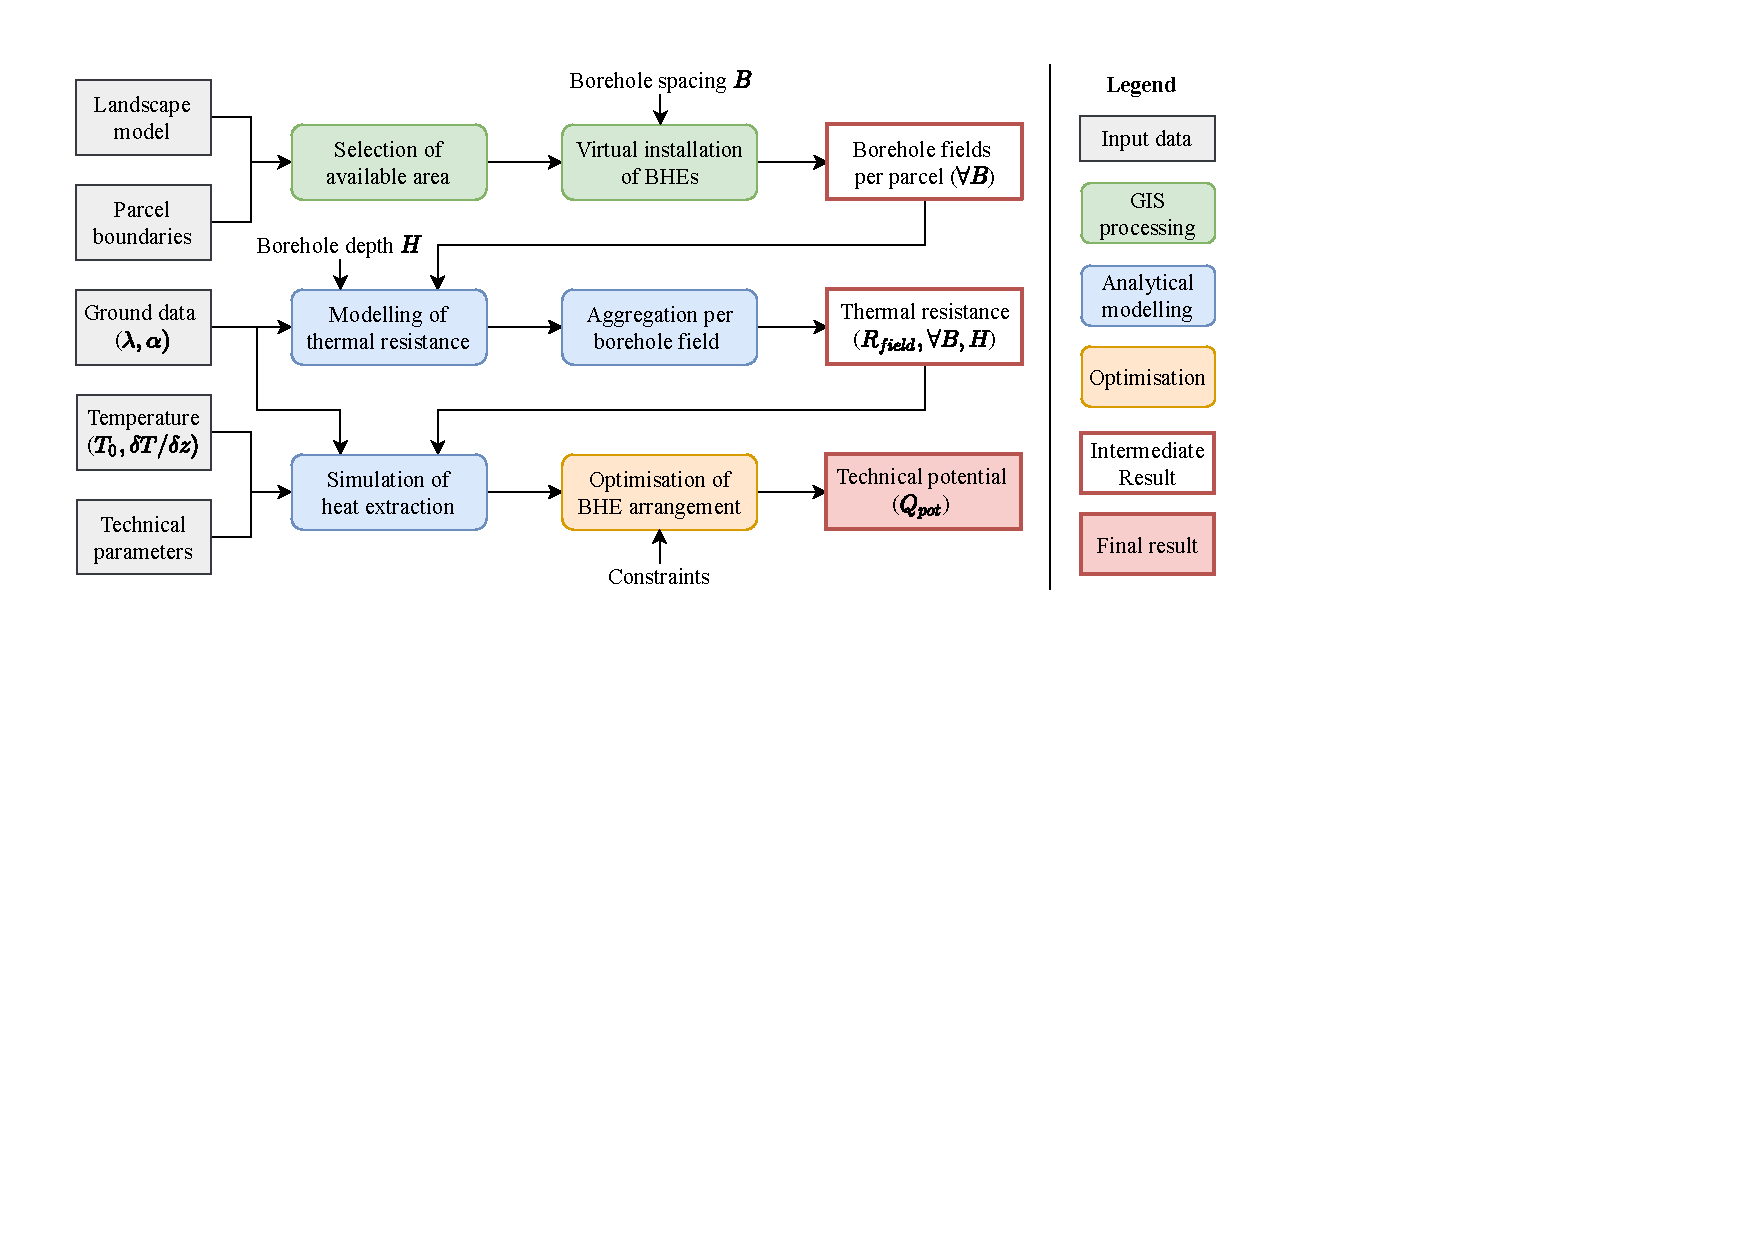
\includegraphics[trim=30 310 250 30,clip,width=1.0\linewidth]{Figs/Geothermal_simplified.pdf}
\caption{Workflow for modelling the technical potential of GSHPs.}
\label{fig:workflow_BHE}
\end{figure}

The proposed method to quantify the technical potential of GSHPs combines 
(i) GIS processing for the virtual installation of BHEs for various density scenarios, where each scenario is defined by a different spacing between adjacent BHEs,
(ii) analytical modelling of the borehole thermal response and its effect on the heat extraction power and the energy potential of the BHEs within each parcel  % borehole thermal resistance and max. operating power and energy
and (iii) an optimisation step to maximise the energy potential of each parcel while assuring a minimum heat extraction power (see Fig.~\ref{fig:workflow_BHE}). % to get the techncial potential
The technical potential represents the annual heat energy that can be extracted from all the BHEs, such that their long-term operation is assured. 
We use a planning horizon ($t_{dim}$) of 50 years as suggested by the geothermal norm of the Swiss society of engineers and architects (SIA)~\cite{sia_sondes_2010}. 
The SIA norm defines the requirements for the dimensioning of shallow GSHPs in Switzerland and sets the technical framework for our work.

\subsection{GIS processing for identifying potential BHE arrangements}
\label{GIS}

To estimate the number of BHEs and their location for different scenarios of installation density, we propose a two-stage GIS-based approach. 
In the first stage, we estimate the available area for the installation of BHEs within each parcel. 
In the second stage, we virtually install BHEs on this available area for each scenarios of installation density, yielding a set of borehole fields. 

To quantify the available area for the installation of BHEs, we combine parcel boundary data with building footprints and other artificial and natural landscape features, obtained from a Topographic Landscape Model (TLM). 
All parcels containing at least one building within their boundaries are considered. 
Parcels without any building inside are neglected, as these parcels neither create a demand for heating nor do they provide any infrastructure to install a GSHP system. 
From the selected parcels, we remove any built-up areas, such as building footprints, roads, railways, traffic-related areas (e.g. parkings, airports) and leisure zones (e.g. sport facilities).
% [FROM DATA] To account for the inaccuracies of the TLM, we apply a tolerance buffer of $1m$ to all objects listed in Section~\ref{GIS}. 
A buffer of $3m$ is removed around all parcels and buildings to assure the minimum distance from a BHE to any building or parcel boundary as specified by the SIA \cite{sia_sondes_2010}.
We also exclude natural and artificial surface water bodies, natural habitat such as forests and wetlands, and protected areas such as national parks.
Fig.~\ref{fig:avail_area_method} shows an example of the excluded objects and the available area within each parcel (blue shading).

\begin{figure}[tb]
    \centering
    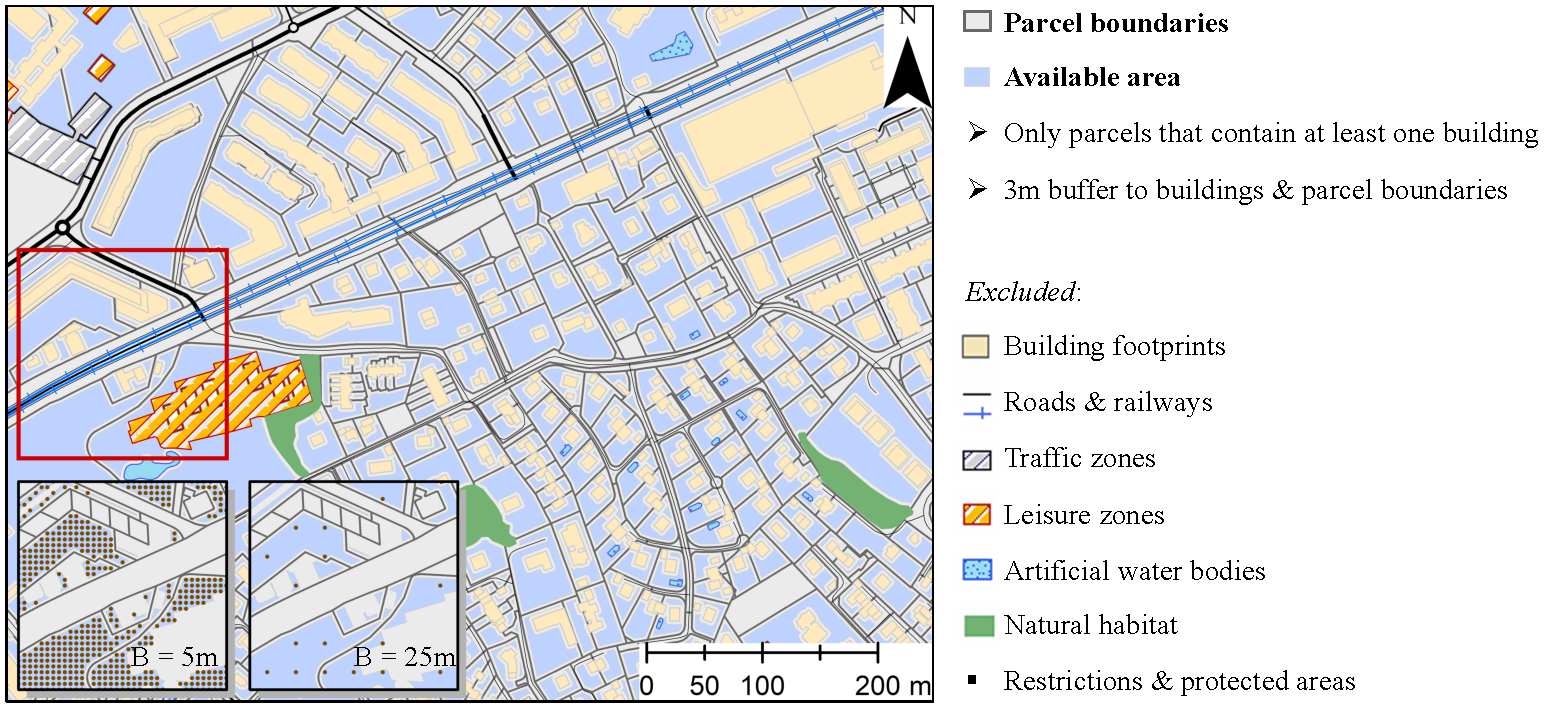
\includegraphics[width=1.0\linewidth]{Figs/avail_area_method.pdf}
    \caption{Sample map showing the parcel boundaries, the available area and the excluded areas according to the Topographic Landscape Model. At the bottom left, the virtual installation of BHEs is shown for two example scenarios (BHE distances $B = 5m, B=25m$) for the area inside the red box.}
    \label{fig:avail_area_method}
\end{figure}

To virtually install BHEs on the available area for all density scenarios, we arrange them on a rectangular grid with varying borehole spacing $B$.
The lower bound for the spacing ($B_{min}$) is given by the SIA norm as $5m$ \cite{sia_sondes_2010}.
The upper bound $B_{max}$ equals half of the maximum borehole depth $H_{max}$, as interactions between BHEs with a spacing exceeding half the borehole depth are small \cite{pahud_geothermal_2002}. 
As thermal interference decreases logarithmically with borehole spacing \cite{eskilson_thermal_1987}, we choose the density scenarios to resemble such a pattern (see Table \ref{tab:data}).
The virtual installation of BHEs for two example scenarios ($B = 5m, B = 25m$) is shown in the bottom left part of Fig.~\ref{fig:avail_area_method}. 
The available area within each parcel yields the separate borehole fields.

\subsection{Analytical model for quantifying the heat extraction potential}
\label{model}

The analytical model introduced by \citet{eskilson_thermal_1987} is used to simulate the borehole thermal response and to derive the heat extraction potential of each field of BHEs.
As the thermal response describes the thermal resistance of a BHE as a function of distance and time, it allows to quantify possible interaction effects between nearby boreholes.
The model represents each BHE as a Finite Line Source (FLS), from which energy is extracted by conductive heat transfer.
Additional heat transfer from groundwater flow is neglected in the model, which may result in some differences between the estimated and the real technical potential.
The simulation of the heat extraction potential requires three types of inputs, namely (i) ground data, (ii) technical parameters and (iii) design variables.
The ground data 
are the thermal conductivity ($\lambda$), the thermal diffusivity ($\alpha$), and the undisturbed ground temperature ($T_g$), which is computed at any depth $z$ from the annual mean surface temperature ($T_0$) and the temperature gradient ($\delta T/\delta z$) using Eq.~\ref{eq:Tg} and subtracting a tolerance of 1 °C (see Chapter \ref{geo_params}).

\begin{comment}
as \cite{sia_sondes_2010}:


\begin{equation}
\label{eq:Tg}
    T_g(z) = T_0 + z \times \frac{\delta T}{\delta z} - 1 ^\circ C
\end{equation}

where the $1 ^\circ C$ is a tolerance that is subtracted to account for uncertainties in the estimation of $T_0$.
\end{comment}

The $\lambda$ and $\alpha$ have been derived from 3D models of the subsurface for various depths \cite{asit_vd_cadastre_2019-1, sitg_cadastre_2019}, the $T_0$ has been estimated from measurement data \cite{assouline_machine_2019} and the $\delta T/\delta z$ is constant (see Table \ref{tab:data}).

The technical parameters include the borehole thermal resistance ($R_b$), the borehole radius ($r_b$) and the annual operating time of the BHEs ($t_{op}$), defined as the typical number of full-load hours of a heat pump at a given altitude \cite{sia_sondes_2010}. 
The design variables are the free parameters in the dimensioning of BHEs and must be selected in order to maximise the technical potential. 
These are the borehole depth ($H$), the borehole spacing ($B$) and the heat extraction rate ($q_{max}$). 
A complete list of all parameters, their units, values/ranges (for spatially varying data) and sources is provided in Table \ref{tab:data}.  

To compute the annual extractable energy for a BHE field ($Q_{field}$), Eq.~(\ref{eq:Q_field}) is used \cite{pahud_geothermal_2002}:

\begin{equation}
\label{eq:Q_field}
    Q_{field}=q_{max} \times t_{op} \times H \times N_B
\end{equation}

where $N_B$ is the number of BHEs in a field with spacing $B$. All $N_B$ BHEs within one field are assumed to have an equal $H$ and $q_{max}$.
As our definition of the potential is independent of the heat demand, we aim to find $q_{max}$ for a given $H$ and $N_B$.
% Such a demand-independent potential has been studied conceptually by \citet{rivera_increased_2017}.
To obtain $q_{max}$, we follow the standard design procedure for geothermal installations \cite{kavanaugh_geothermal_2014, spitler_vertical_2016, pahud_geothermal_2002}. 
According to this procedure, GSHP systems for heating are designed such that the mean temperature of the heat carrier fluid ($T_{mf}$) inside the borehole remains above a minimum value $T_{mf, min}$, given as $-1.5 ^\circ C$ in the norm \cite{sia_sondes_2010}, throughout $t_{dim}$. 
Rearranging the expression for $T_{mf, min}$, we compute $q_{max}$ for each BHE field and each given $B$ and $H$ as shown in Eq.~(\ref{eq:q_max}) (cf. \cite{pahud_geothermal_2002}):

\begin{equation}
\label{eq:q_max}
    q_{max} = \frac{T_g(\frac{H}{2}) - T_{mf, min}}{\overline{w}(R_{LT}(r_b, H) + R_{field}(B, H)) + w_{seas} R_{seas} + R_b}
\end{equation}


where $T_g$ is given in Eq.~(\ref{eq:Tg}); $T_{mf, min}$ is constant (Table~\ref{tab:data});
$\overline{w}$ is the annual mean load of the GSHP system (as fraction of the full load), and is given by $\overline{w} = t_{op}/ (365 \times 24h)$;
$R_{LT}$ is the long-term thermal resistance of a BHE (\ref{app:models}), computed at the borehole wall, i.e. at a radial distance $r_b$ (Table~\ref{tab:data});
$R_{field}$ (Eq.~(\ref{eq:R_field})) is the average long-term thermal resistance of a BHE field; % (Eq.~(\ref{eq:R_field})); 
$w_{seas}$  (Eq.~(\ref{eq:w_seas})) and $R_{seas}$ (\ref{app:models}) are the seasonal mean system load % (Eq.~(\ref{eq:w_seas})) 
and the seasonal thermal resistance, respectively; 
and $R_b$, the borehole thermal resistance, is constant (Table~\ref{tab:data}).
The expressions for $R_{LT}$ and $R_{seas}$, which depend on $\lambda$ and $\alpha$, are provided in \ref{app:models}. 

According to the superposition principle \cite{eskilson_thermal_1987}, the long-term thermal resistance of BHEs in a field may be estimated by summing 
% the $R_{LT}$ at the borehole wall, i.e. at a radial distance $r_b$, and 
the $R_{LT}$ at each $r_{i,B} \leq H$, where $r_{i,B}$ is the distance to the $i^{th}$ nearby BHE for a scenario $B$.
For any $r > H$, there is a negligible effect on the thermal response \cite{pahud_geothermal_2002}. 
The $R_{field}$ is the average thermal resistance for $N_B$ BHEs in a field, given by:

\begin{equation}
\label{eq:R_field}
    R_{field}(H, B) = \frac{1}{N_B} \sum_{i=1}^{N_B} \sum_{r_{i,B} \leq H} R_{LT}(r_{i,B}, H)
\end{equation}

To limit the number of possible combinations of $B$ and $H$, we assume that the BHE spacing and depth within a field equals that of all neighboring fields within a radius of $H$.
% The error introduced by this assumption will be assessed in Section \ref{results}. 
We further assume the ground data to be constant within each field, which holds for over 99\% of the cases. 

The effect of the seasonal variation of the GSHP system load on $q_{max}$ is modelled as the maximum of a sinusoidal heat extraction with a periodicity of 1 year and an amplitude $w_{seas}$ (cf. \cite{pahud_geothermal_2002}). 
We derive $w_{seas}$ from the Heating Degree Days (HDD) describing the monthly heating profile of a given location.
As Fig.~\ref{fig:w_seas} shows, the monthly mean GSHP system load $\overline{w}_m$ (blue bars, as fraction of the full load), weighted by the HDD, resembles a sinusoid superimposed on $\overline{w}$ (red line).
We thus propose here to approximate $w_{seas}$ by subtracting $\overline{w}$ from the mean system load in the month with the maximum heating demand (typically January in Switzerland):

\begin{equation}
\label{eq:w_seas}
    w_{seas} = w_{hdd,max} \times \frac{t_{op}}{31\times24h} - \overline{w} % OR: q_{seas} = 12 \times w_{hdd} \times \overline{q}
\end{equation}

where $w_{hdd,max}$ is the highest relative HDD, defined as:
\begin{equation}
\label{eq:w_HDD}
    w_{hdd,max} = 1.05 \  \frac{HDD_{max}}{\sum HDD}
\end{equation}

$HDD_{max}$ is the maximum monthly HDD, $\sum HDD$ is the annual sum, and a buffer of 5\% (hence the factor 1.05) is multiplied with this ratio to avoid an underestimation of $w_{hdd,max}$.
The computation of the HDD from the ambient air temperature is detailed in \ref{app:HDD}.

\begin{figure}[tb]
\centering
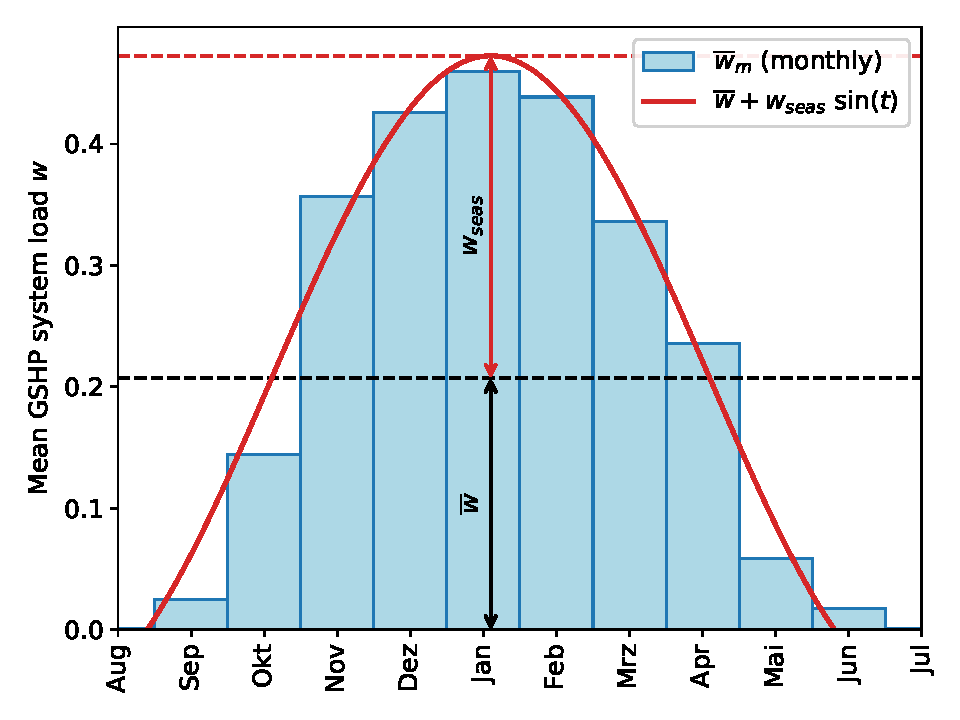
\includegraphics[width=0.6\linewidth]{Figs/w_seas.pdf} 
\caption{Example of the monthly mean GSHP system load ($\overline{w}$, blue bars, as fraction of the full load) and its sinusoidal approximation ($\overline{w} + w_{seas} \ \sin(t)$, red line), based on the HDD of a representative location for western Switzerland (weather station of Pully) with a heating season of $\sim 6$ months.}
\label{fig:w_seas}
\end{figure}

\begin{comment} 
\begin{equation}
\label{eq:q}
    \overline{q} = q_{max} \times \frac{t_{op}}{365\times24}, \quad q_{seas} = q_{max} \times w_{hdd} \times \frac{t_{op}}{31\times24} - \overline{q}  % OR: q_{seas} = 12 \times w_{hdd} \times \overline{q}
\end{equation}
\end{comment} 

\subsection{Optimisation}
\label{optimisation}

The aim of the optimisation is to select, for each BHE field separately, the borehole density $B_{opt}$ and borehole depth $H_{opt}$ that maximise $Q_{field}$, yielding the technical potential $Q_{pot}$.
This optimisation is constrained by two factors: the maximum BHE depth $H_{max}$ and the minimum heat extraction rate $q_{min}$.
The $H_{max}$ is limited by local conditions and regulations (see Section \ref{data_geo}).
The $q_{min}$ represents a proxy of the economic feasibility of a GSHP system. 
We propose to derive $q_{min}$ from the nominal heat extraction rate $q_{nom}$, which represents current installation practices. 
Based on the data provided in the SIA norm, $q_{nom}$ can be approximated as shown in Eq.~\ref{eq:q_nom}.

\begin{comment}
as \cite{sia_sondes_2010}:

\begin{equation}
\label{eq:q_nom}
    q_{nom} \approx \frac{T_g - T_{mf, min}}{11.5} \ \left( 10.6 \lambda + 11.2 + 2 \left( \frac{\lambda}{\alpha} - 2 \right) \right)
\end{equation}
\end{comment}

To soften this constraint, we set $q_{min}$ at 80\% of $q_{nom}$, which corresponds to the expected power loss for domestic installations with multiple BHEs under the given operating conditions \cite{sia_sondes_2010}.
The optimisation problem may hence be formulated as: 
%
\begin{equation}
\label{eq:optimisation}
    Q_{pot} = \max_{B, H} \; Q_{field} \quad \quad \text{subject to} \; H \leq H_{max}, \; q_{max} \geq 0.8 \ q_{nom}
\end{equation}

\begin{landscape}
\begin{table}[b]
\footnotesize
\caption{Description of variables and parameters used in this work. The ground data and $H_{max}$ are specific for the case study area and will be detailed in Section \ref{case_study}. Values in brackets represent averages across the study region.}
\centering
% \rotatebox{90}{
\begin{tabular}{clllll}
\hline
\textbf{Type} & \textbf{Symbol}             & \textbf{Unit} & \textbf{Description}           & \textbf{Value/range} & \textbf{Source} \\ \hline
\multirowcell{4}{Ground \\ data}
& $\lambda$           & $W/mK$        & Thermal conductivity         & $1.6-3.0$ (2.4) 
& ASIT-VD \cite{asit_vd_cadastre_2019-1}, SITG \cite{sitg_cadastre_2019}      \\
& $\alpha$            & $\mu m^2/s$       & Thermal diffusivity          & $0.6-1.4$ (1.1)   
& ASIT-VD \cite{asit_vd_cadastre_2019-1}, SITG \cite{sitg_cadastre_2019}            \\
& $T_0$               & $^\circ C$    & Surface temperature          & $8 - 11$ (10.4)  
& \citet{assouline_machine_2019}              \\
& $\delta T/\delta z$ & $K/m$         & Temperature gradient         & 0.03     
& SIA norm \cite{sia_sondes_2010} \\
\hline
\multirowcell{6}{Technical \\ parameters}
& $T_{mf, min}$      & $^\circ C$    & Minimum fluid temperature     & $- 1.5$      
& SIA norm \cite{sia_sondes_2010}  \\
& $t_{dim}$          & $a$           & Planning horizon              & $50$               
& SIA norm \cite{sia_sondes_2010}  \\ 
& $t_{op}$           & $h$           & Annual operation time         & $1800-2000$ (1830)
& SIA norm \cite{sia_sondes_2010}  \\
% & $t_{peak}$         & $d$           & Duration of extraction pulse  & $1$ day        
% & \citet{pahud_geothermal_2002}  \\ 
& $r_b$              & $m$           & Borehole radius               & $0.065$           
& \citet{perego_techno-economic_2019, miglani_methodology_2018} \\
& $R_b$            & $mK/W$        & Effective borehole resistance & $0.15$     
& \citet{rivera_increased_2017}  \\ 
& $w_{hdd, max}$   & -             & Maximum HDD weight            & $0.16-0.20$ (0.19)
& Eq.~(\ref{eq:w_HDD}), \ref{app:HDD} \\
\hline
\multirowcell{4}{Design \\ variables}
& $q_{max}$          & $W/m$         & Maximum heat extraction rate  & \textit{Target variable} \\
& $H$                & $m$           & Borehole depth                & \{50, 100, 150, 200\}    
& Derived from \cite{asit_vd_cadastre_2019-1, sitg_cadastre_2019} \\
& $B$                & $m$           & Spacing between BHEs          & \makecell[tl]{\{5,7,10,15,20,25, \\ \hspace{3mm}30,40,50,70,100\}}
& Derived from $H_{max}$ \cite{pahud_geothermal_2002} \\ 
% & $D$             & $m$           & Distance of surface to outlet          & $2$ & \citet{pahud_geothermal_2002} \\
\hline
\multirowcell{3}{Optimisation \\ constraints}
& $q_{nom}$          & $W/m$         & Nominal heat extraction rate  & $30-45$ (41.5)
& SIA norm \cite{sia_sondes_2010} \\
& $H_{max}$          & $m$           & Maximum borehole depth       & \makecell[tl]{Permitted: $200$ \\ Limited: $150$}
& Derived from \cite{asit_vd_cadastre_2019-1, sitg_cadastre_2019} \\
\hline
\multirowcell{4}{Outputs}
& $N_B$              & -             & Number of boreholes per field     & $f(B)$  
& Section \ref{model} \\
& $Q_{field}$        & $Wh$          & Extractable energy of BHE field   & $f(H,B)$
& Eq.~(\ref{eq:Q_field}), Section \ref{model} \\
& $H_{opt}, B_{opt}$ & $m$           & Optimal borehole depth, spacing   & $\in H,B$
& Section \ref{optimisation} \\
& $Q_{pot}$          & $Wh$          & Technical potential               & $Q_{field}$($H_{opt}$, $B_{opt}$)
& Eq.~(\ref{eq:optimisation}), Section \ref{optimisation} \\
\hline
\end{tabular}
% }
\label{tab:data}
\end{table}

\end{landscape}

\subsection{Case study}
\label{case_study}

To demonstrate the performance of the proposed method at regional scale, we apply it to the cantons of Vaud and Geneva in Switzerland. 
The selected cantons are well-suited for this study as they consist of both urban and rural zones, already contain a large number of BHEs
and offer high-resolution landscape data as well as geothermal cadastres with information for the planning of GSHP systems.
Furthermore, the annual heat demand for the cantons is available from \citet{schneider_spatialtemporal_2017} at a pixel resolution of $200 \times 200 m^2$. 
This data is used to assess potential surpluses or deficits of geothermal heat generation.
For this assessment, we assume that all GSHPs are sized appropriately and have a coefficient of performance (COP) of 4.5 as suggested by \citet{galgaro_empirical_2015}.

The case study covers a surface of around 1600 $km^2$ in the western part of the Swiss plateau that contains over 250,000 buildings. 
Its largest cities are Geneva and Lausanne at the borders of Lake Geneva (see Fig.~\ref{fig:lims}).
Geologically, the plateau is situated in the alpine Molasse Basin between the Jura in the north and the Prealps in the south. 
Its shallow subsurface ($< 400m$) consists primarily of a layer of unconsolidated Quarternary deposits, with a thickness of $0 - 150m$, which is located on top of the clastic sedimentary rocks of the Swiss molasse \cite{allenbach_geomol_2105}. %

\begin{figure}[!ht] % !
\centering
\makebox[\linewidth][c]{
\begin{subfigure}{.49\textwidth}
  \centering
  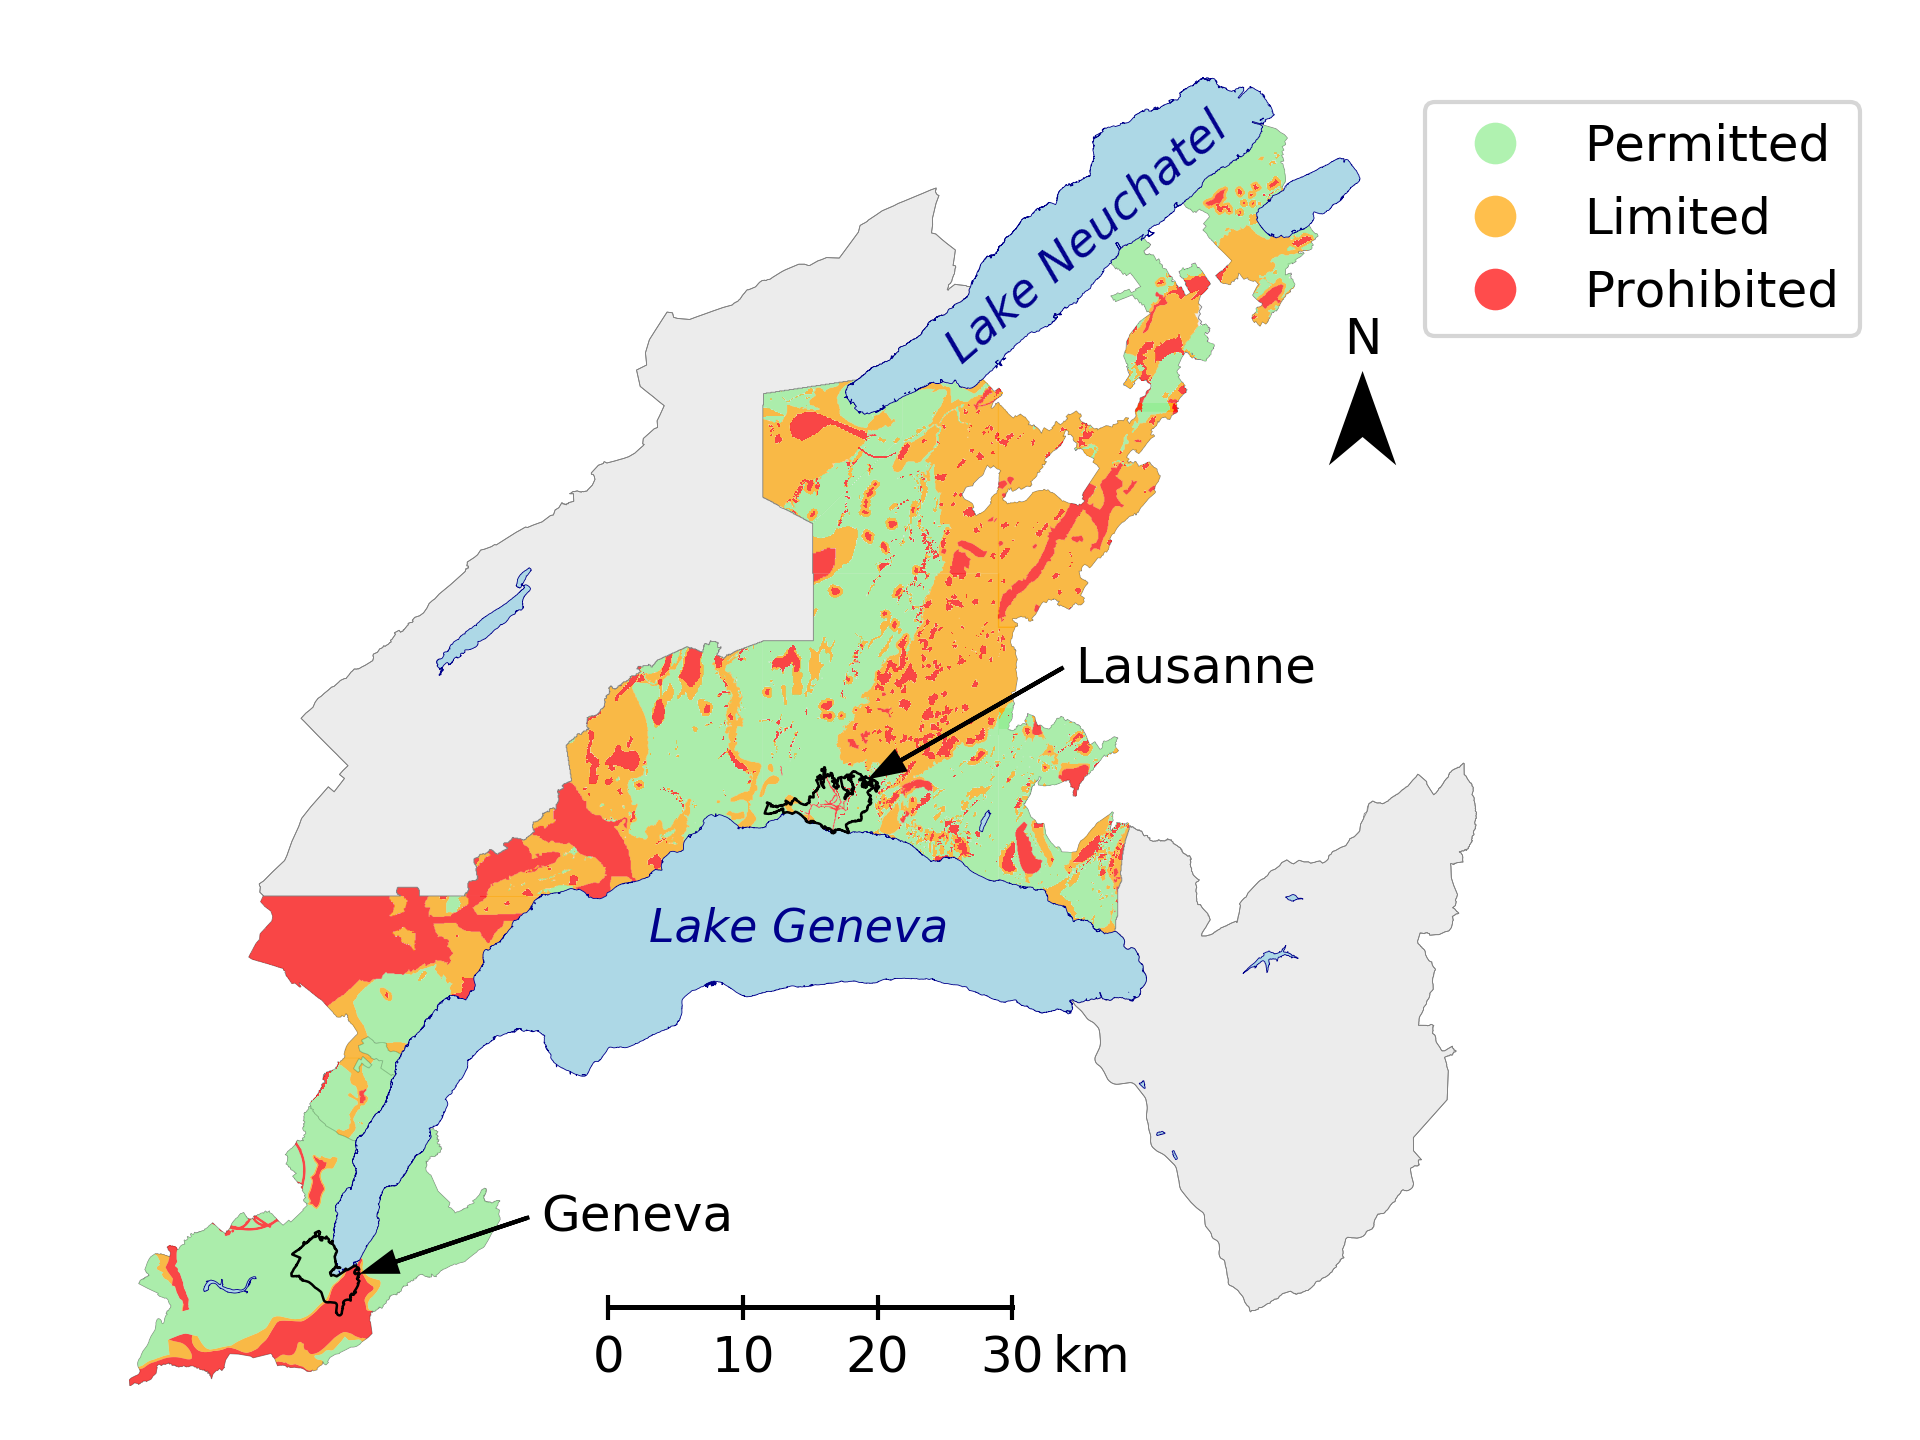
\includegraphics[width=\linewidth]{Figs/ADM_ZONES_w_NAMES.png}  
  \subcaption{}
  \label{fig:lims}
\end{subfigure}
\begin{subfigure}{.49\textwidth}
  \centering
  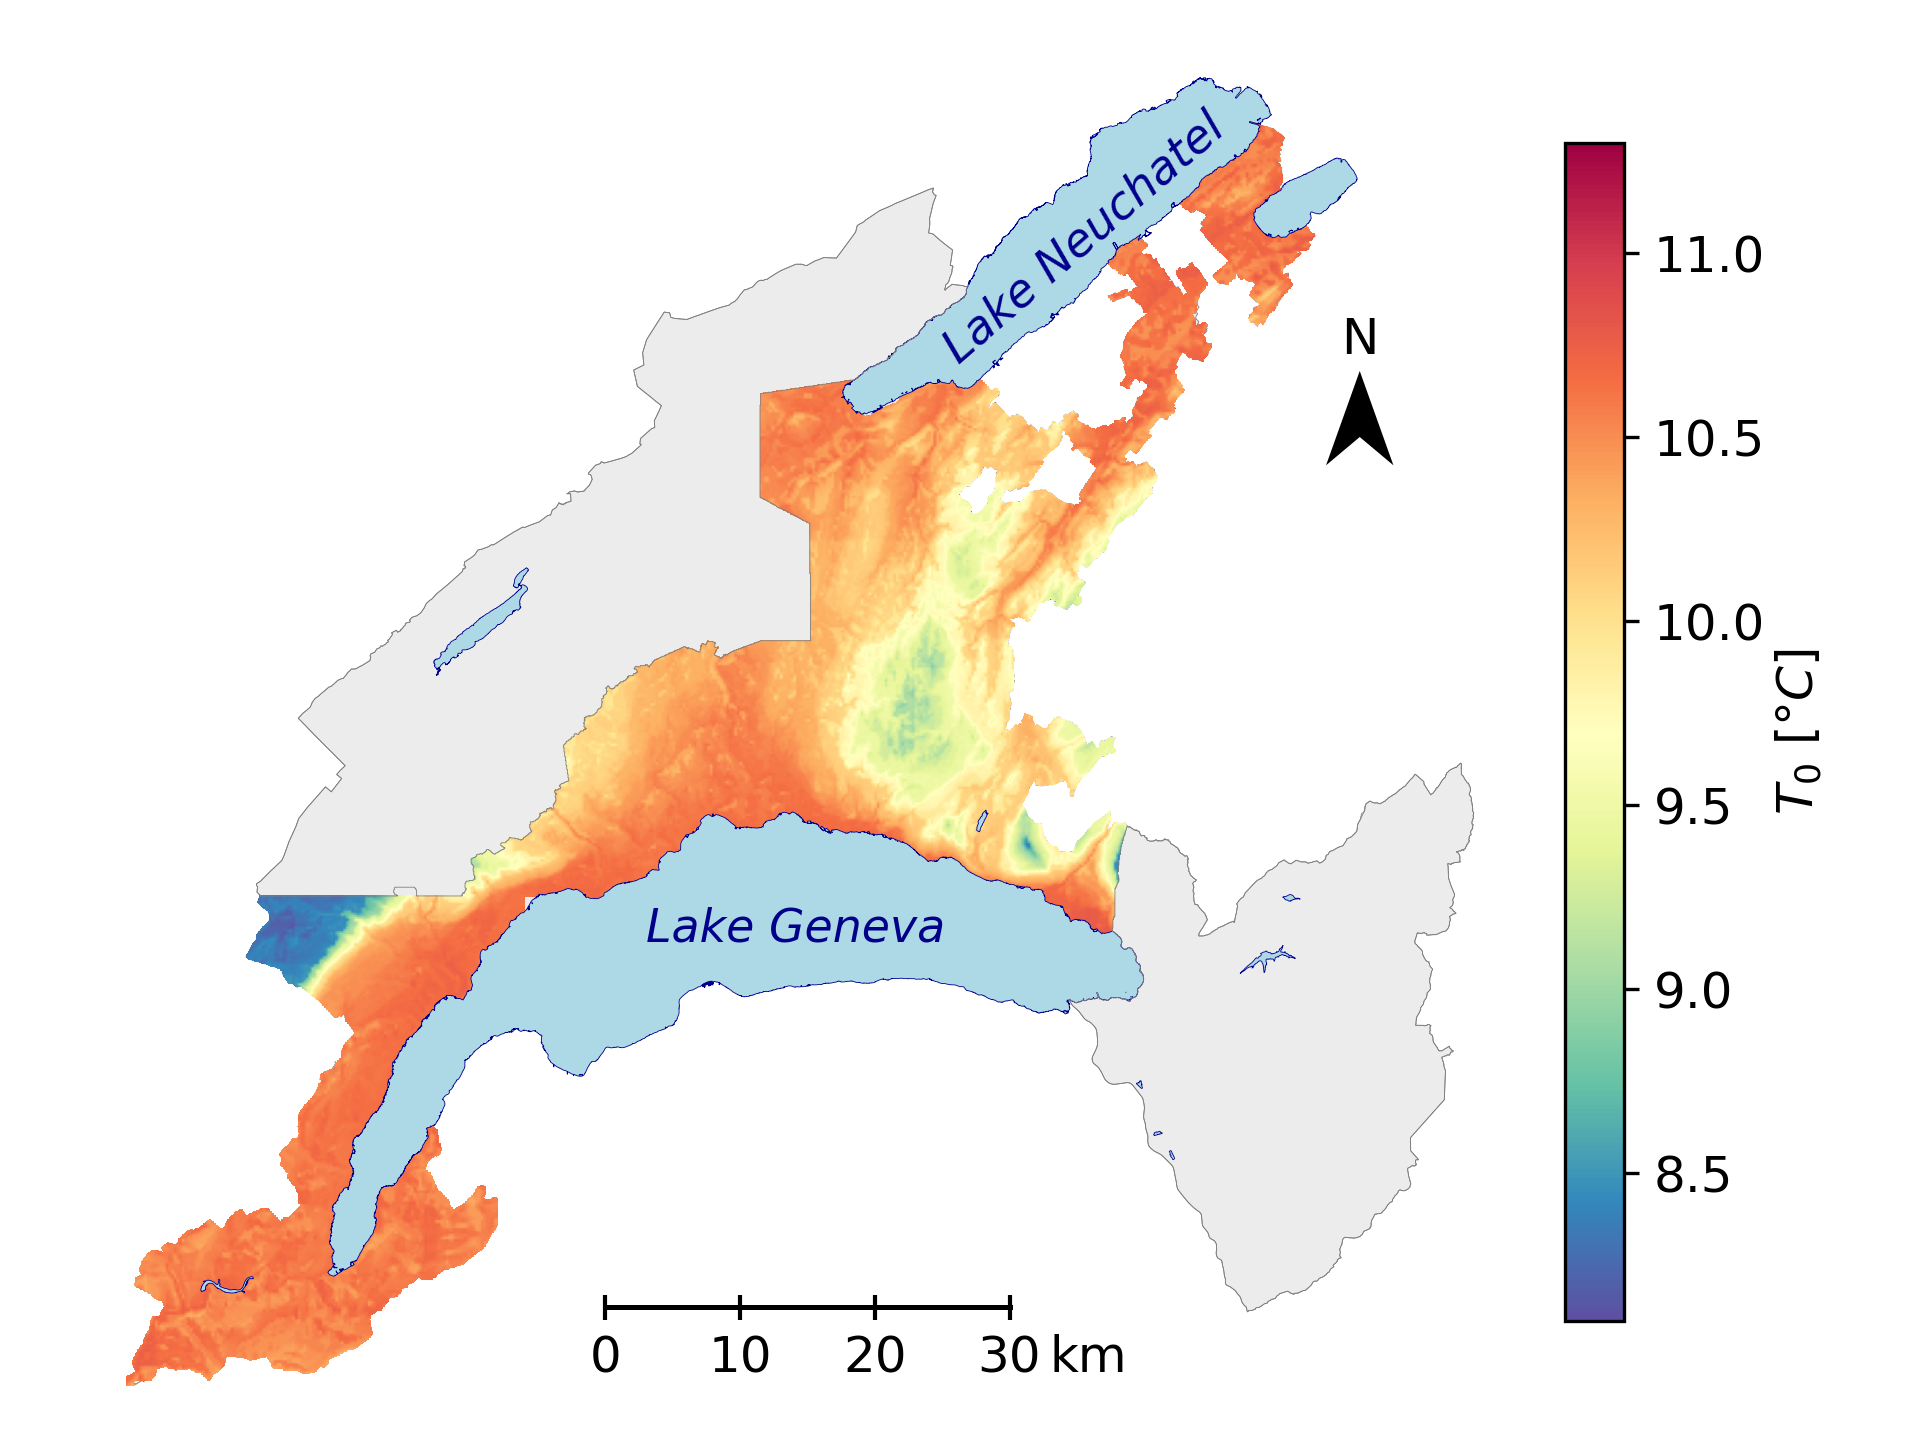
\includegraphics[width=\linewidth]{Figs/T_surface_1m.png} 
  \subcaption{}
  \label{fig:T0}
\end{subfigure}
} \\
\makebox[\linewidth][c]{
\begin{subfigure}{.49\textwidth}
  \centering
  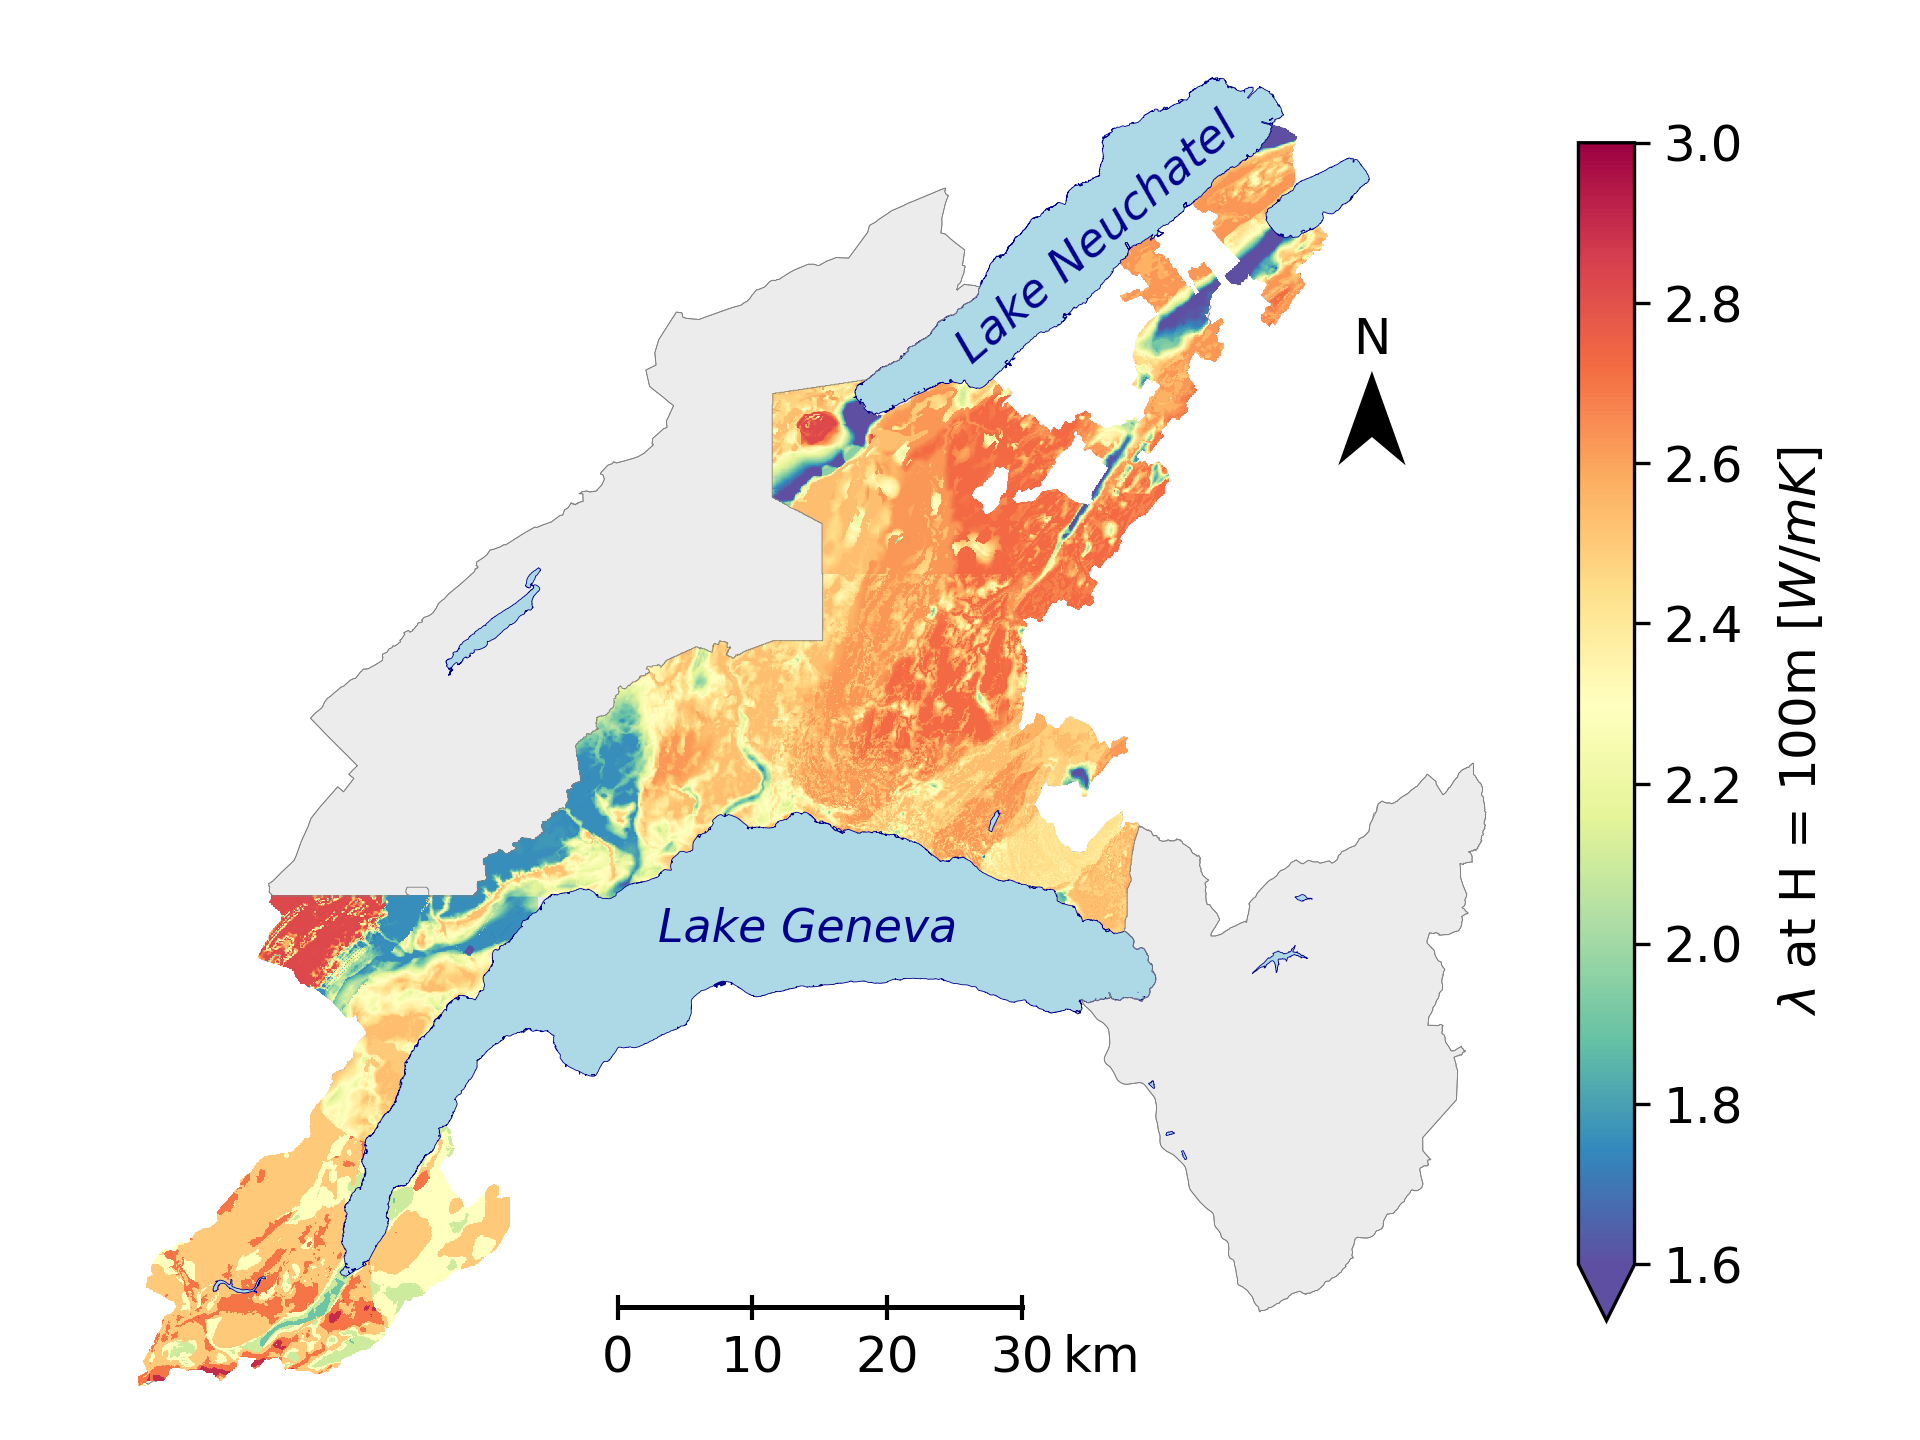
\includegraphics[width=\linewidth]{Figs/Lambda_100.png}
  \subcaption{}
  \label{fig:lambda}
\end{subfigure}
\begin{subfigure}{.49\textwidth}
  \centering
  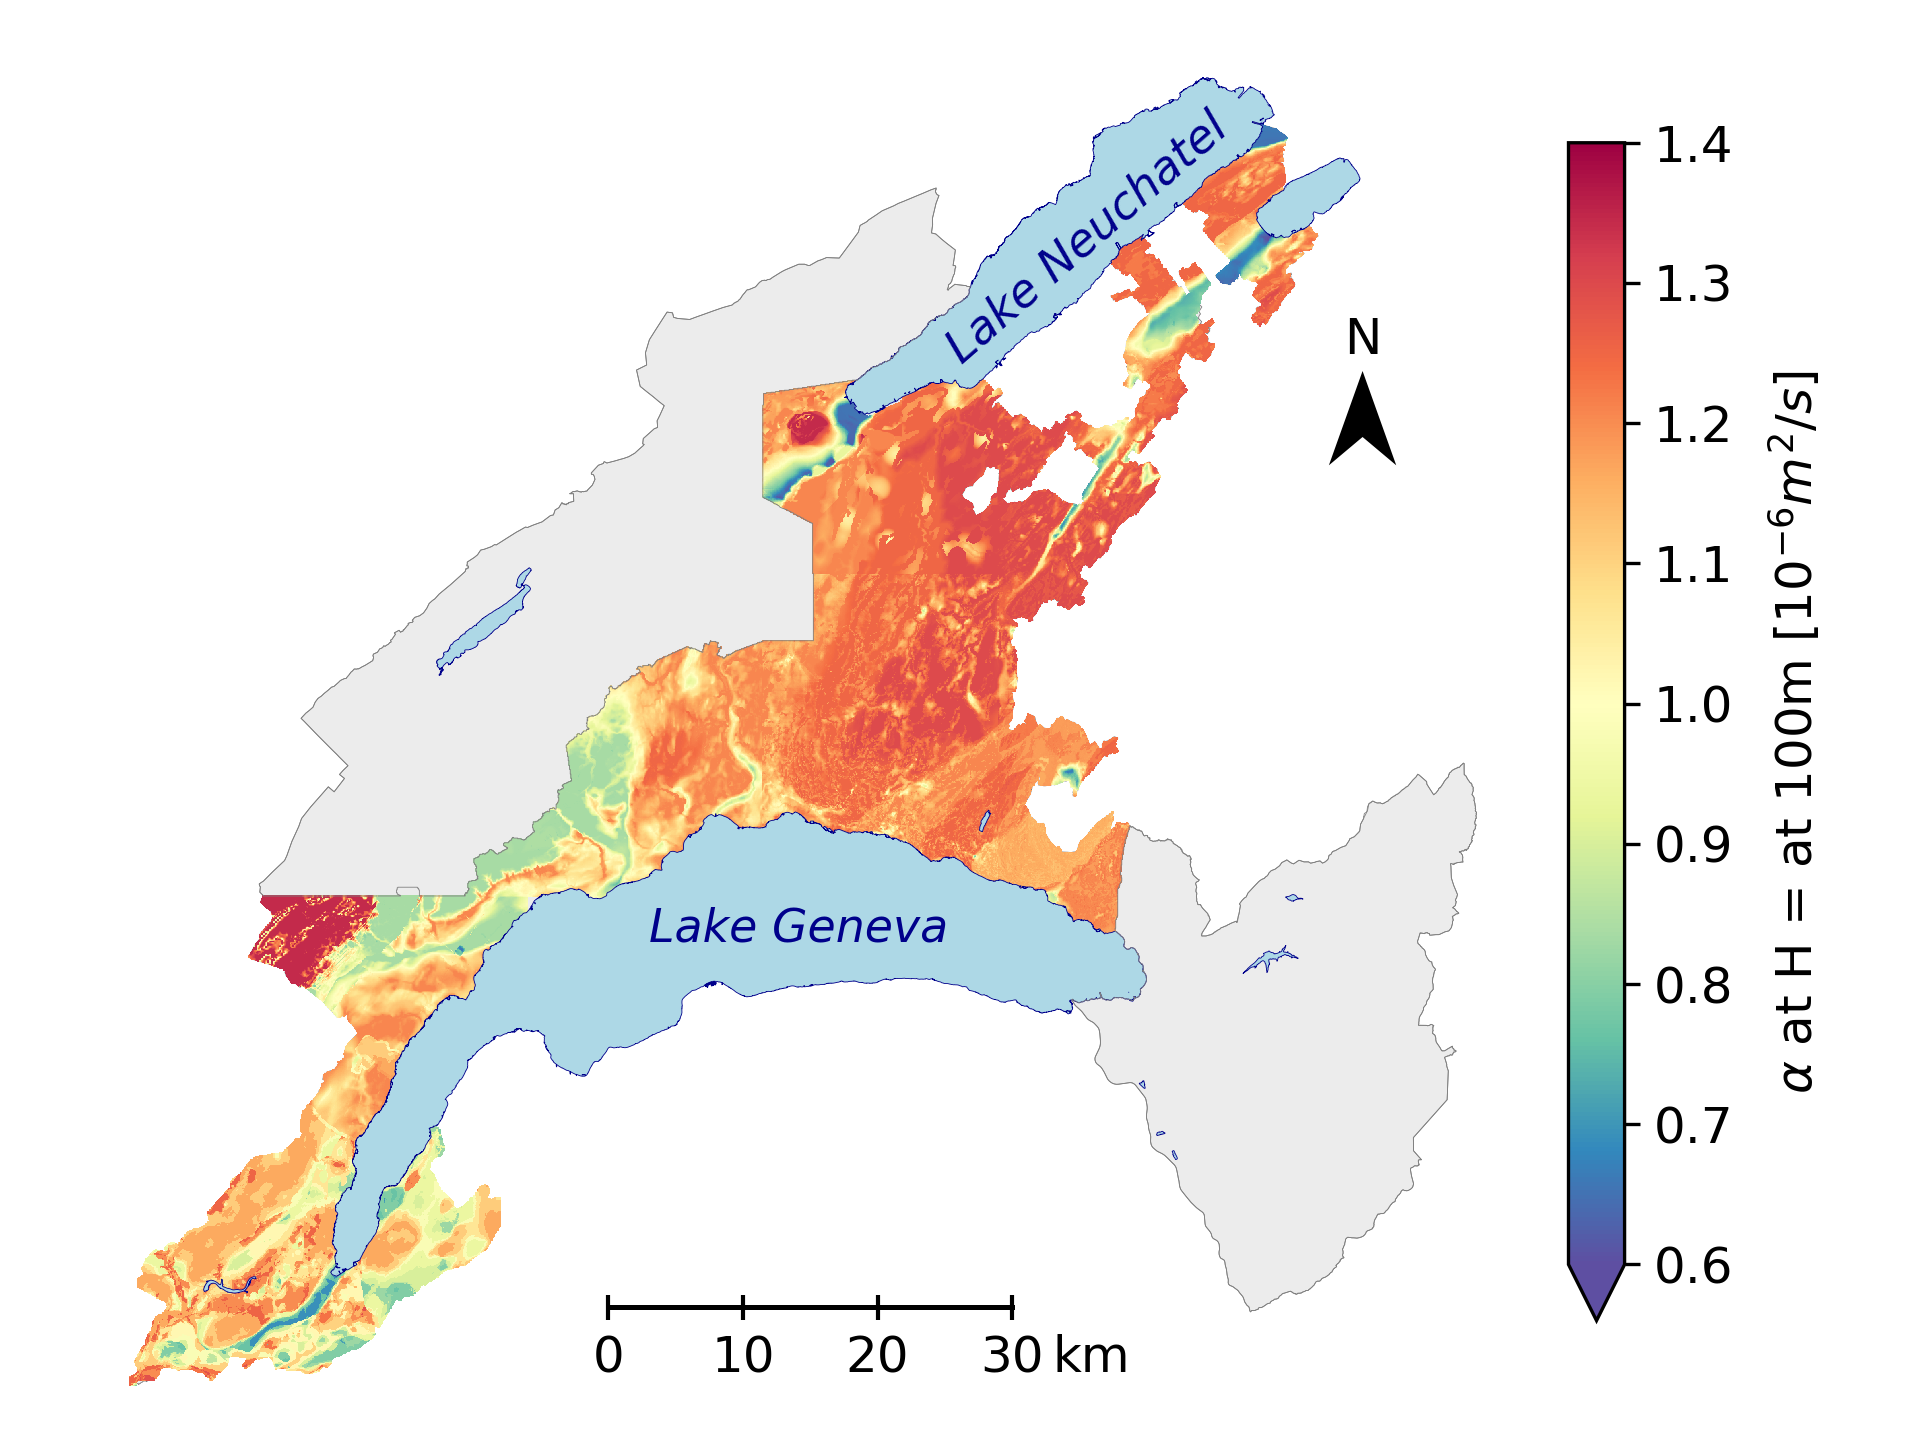
\includegraphics[width=\linewidth]{Figs/Alpha_100.png}
  \subcaption{}
  \label{fig:alpha}
\end{subfigure}
}
\caption{Regional variation of ground data in the case study region. a) Restriction zones for geothermal installations, b) Ground surface temperature at $1m$ depth, from \citet{assouline_machine_2019}, c) Thermal conductivity ($\lambda$) and d) Thermal diffusivity ($\alpha$) based on the geothermal cadastres \cite{asit_vd_cadastre_2019, sitg_cadastre_2019}. Grey zones are outside the study area.}
\label{fig:data}
\end{figure}

\section{Results}
\label{results}

\subsection{Available area and borehole fields}

The application of our method to the case study region in western Switzerland suggests that an area of $284 km^2$ may be available for the installation of BHEs on 80,000 of the 100,000 parcels (property units).
The percentage of available area varies widely within the case study region, as the aggregation of the parcels to pixels of $200 \times 200 m^2$ shows (Fig.~\ref{fig:avail_area}).
The available area is small in dense urban areas, particularly at the borders of Lake Geneva, and drops below 10\% in the city centers of Lausanne and Geneva. 
In rural areas, the spread is much larger, varying widely between nearly 0\% and 100\%. 
This is due to the fact that rural parcels are spaced far apart and may cover multiple pixels. 
% Consequently, some pixels contain only a negligible fraction of available area, while in other pixels the entire area may be available for installing BHEs.

The results yield BHE fields for each density scenario $B$ (see Table~\ref{tab:data}), an example of which ($B = 7m$) is shown in Fig.~\ref{fig:R_field_sample}.
This scenario equals the current recommendations for the distance between BHEs \cite{miglani_methodology_2018}, but it results in unrealistically high numbers of BHEs in large fields. 
Borehole spacings of around $H/2$ ($B=50-100m$), on the other hand, represent conservative scenarios that leave many fields unused. 

\begin{figure}[tb]
\centering
\makebox[\linewidth][c]{
\begin{subfigure}{\textwidth}
  \centering
  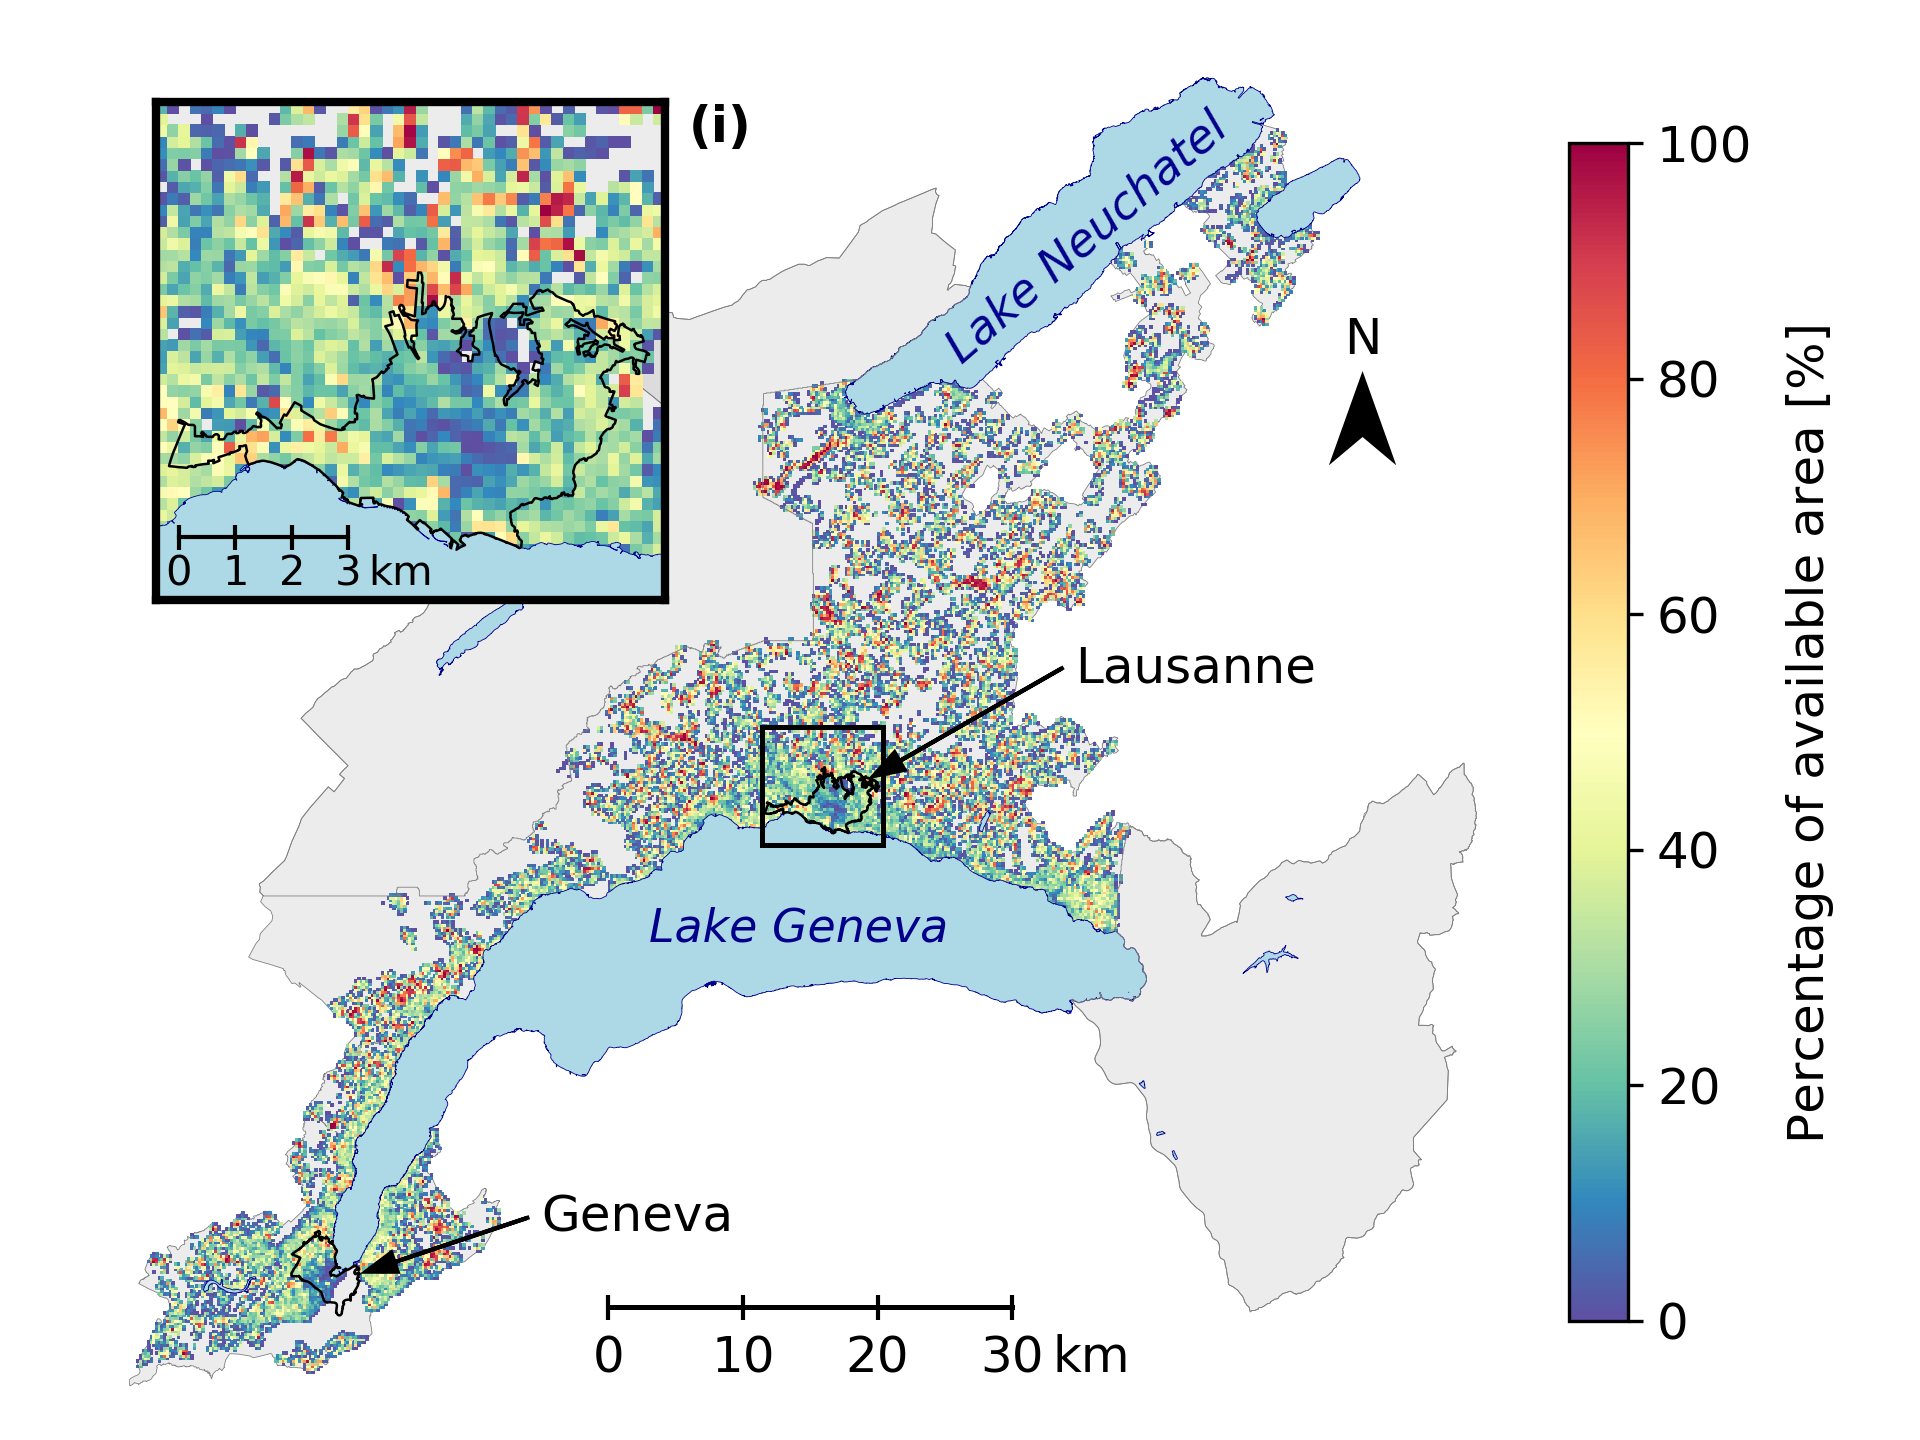
\includegraphics[width=.7\linewidth]{Figs/Free_area_perc.png} 
\end{subfigure}
}
\caption{Percentage of available area for pixels of $200 \times 200m^2$, obtained as the sum of the available area of all parcels within a pixel, relative to its area of $40,000 m^2$. The inset (i) shows a zoom into the area around Lausanne.}
\label{fig:avail_area}
\end{figure}

\subsection{Thermal resistance of interacting boreholes}

The simulation results show that the thermal resistance $R_{field}$, representing the interactions between boreholes, 
varies with the parcel shape and size. 
As the thermal resistance decreases logarithmically with distance to a borehole, the average $R_{field}$ is strongly influenced by the average number of immediately neighboring BHEs within a parcel.
Consequently, large fields have a higher $R_{field}$ than small or oddly shaped ones (see colour gradient in Fig.~\ref{fig:R_field_sample} for $B=7m,H=50m$).
In particular, $R_{field}$ is small in fields located next to roads or other unavailable areas, where no BHEs can be installed (white spaces in Fig.~\ref{fig:R_field_sample}). 
%
The relationship between $R_{field}$ and the borehole spacing also causes $R_{field}$ to fall steeply as $B$ increases, for any $H$ (see Fig.~\ref{fig:R_field_mean}).
Fig.~\ref{fig:R_field_mean} further shows that $R_{field}$ increases non-linearly with $H$, which means that decreasing $H$ reduces interactions between BHEs.
%
For $H = 50m$, $R_{field}$ drops below the long-term resistance of the BHE itself ($R_{LT}$, dashed line) near $B = 11.5m$, at which point the field resistance is no longer dominating the long-term effects, and flattens out near $B = 25m$. 
The same behaviour is found for $H \geq 100m$, but at spacings of $20m$ and $50m$, respectively.

\begin{figure}[tb]
\centering
\makebox[\linewidth][c]{
\begin{subfigure}{.49\textwidth}
  \centering
  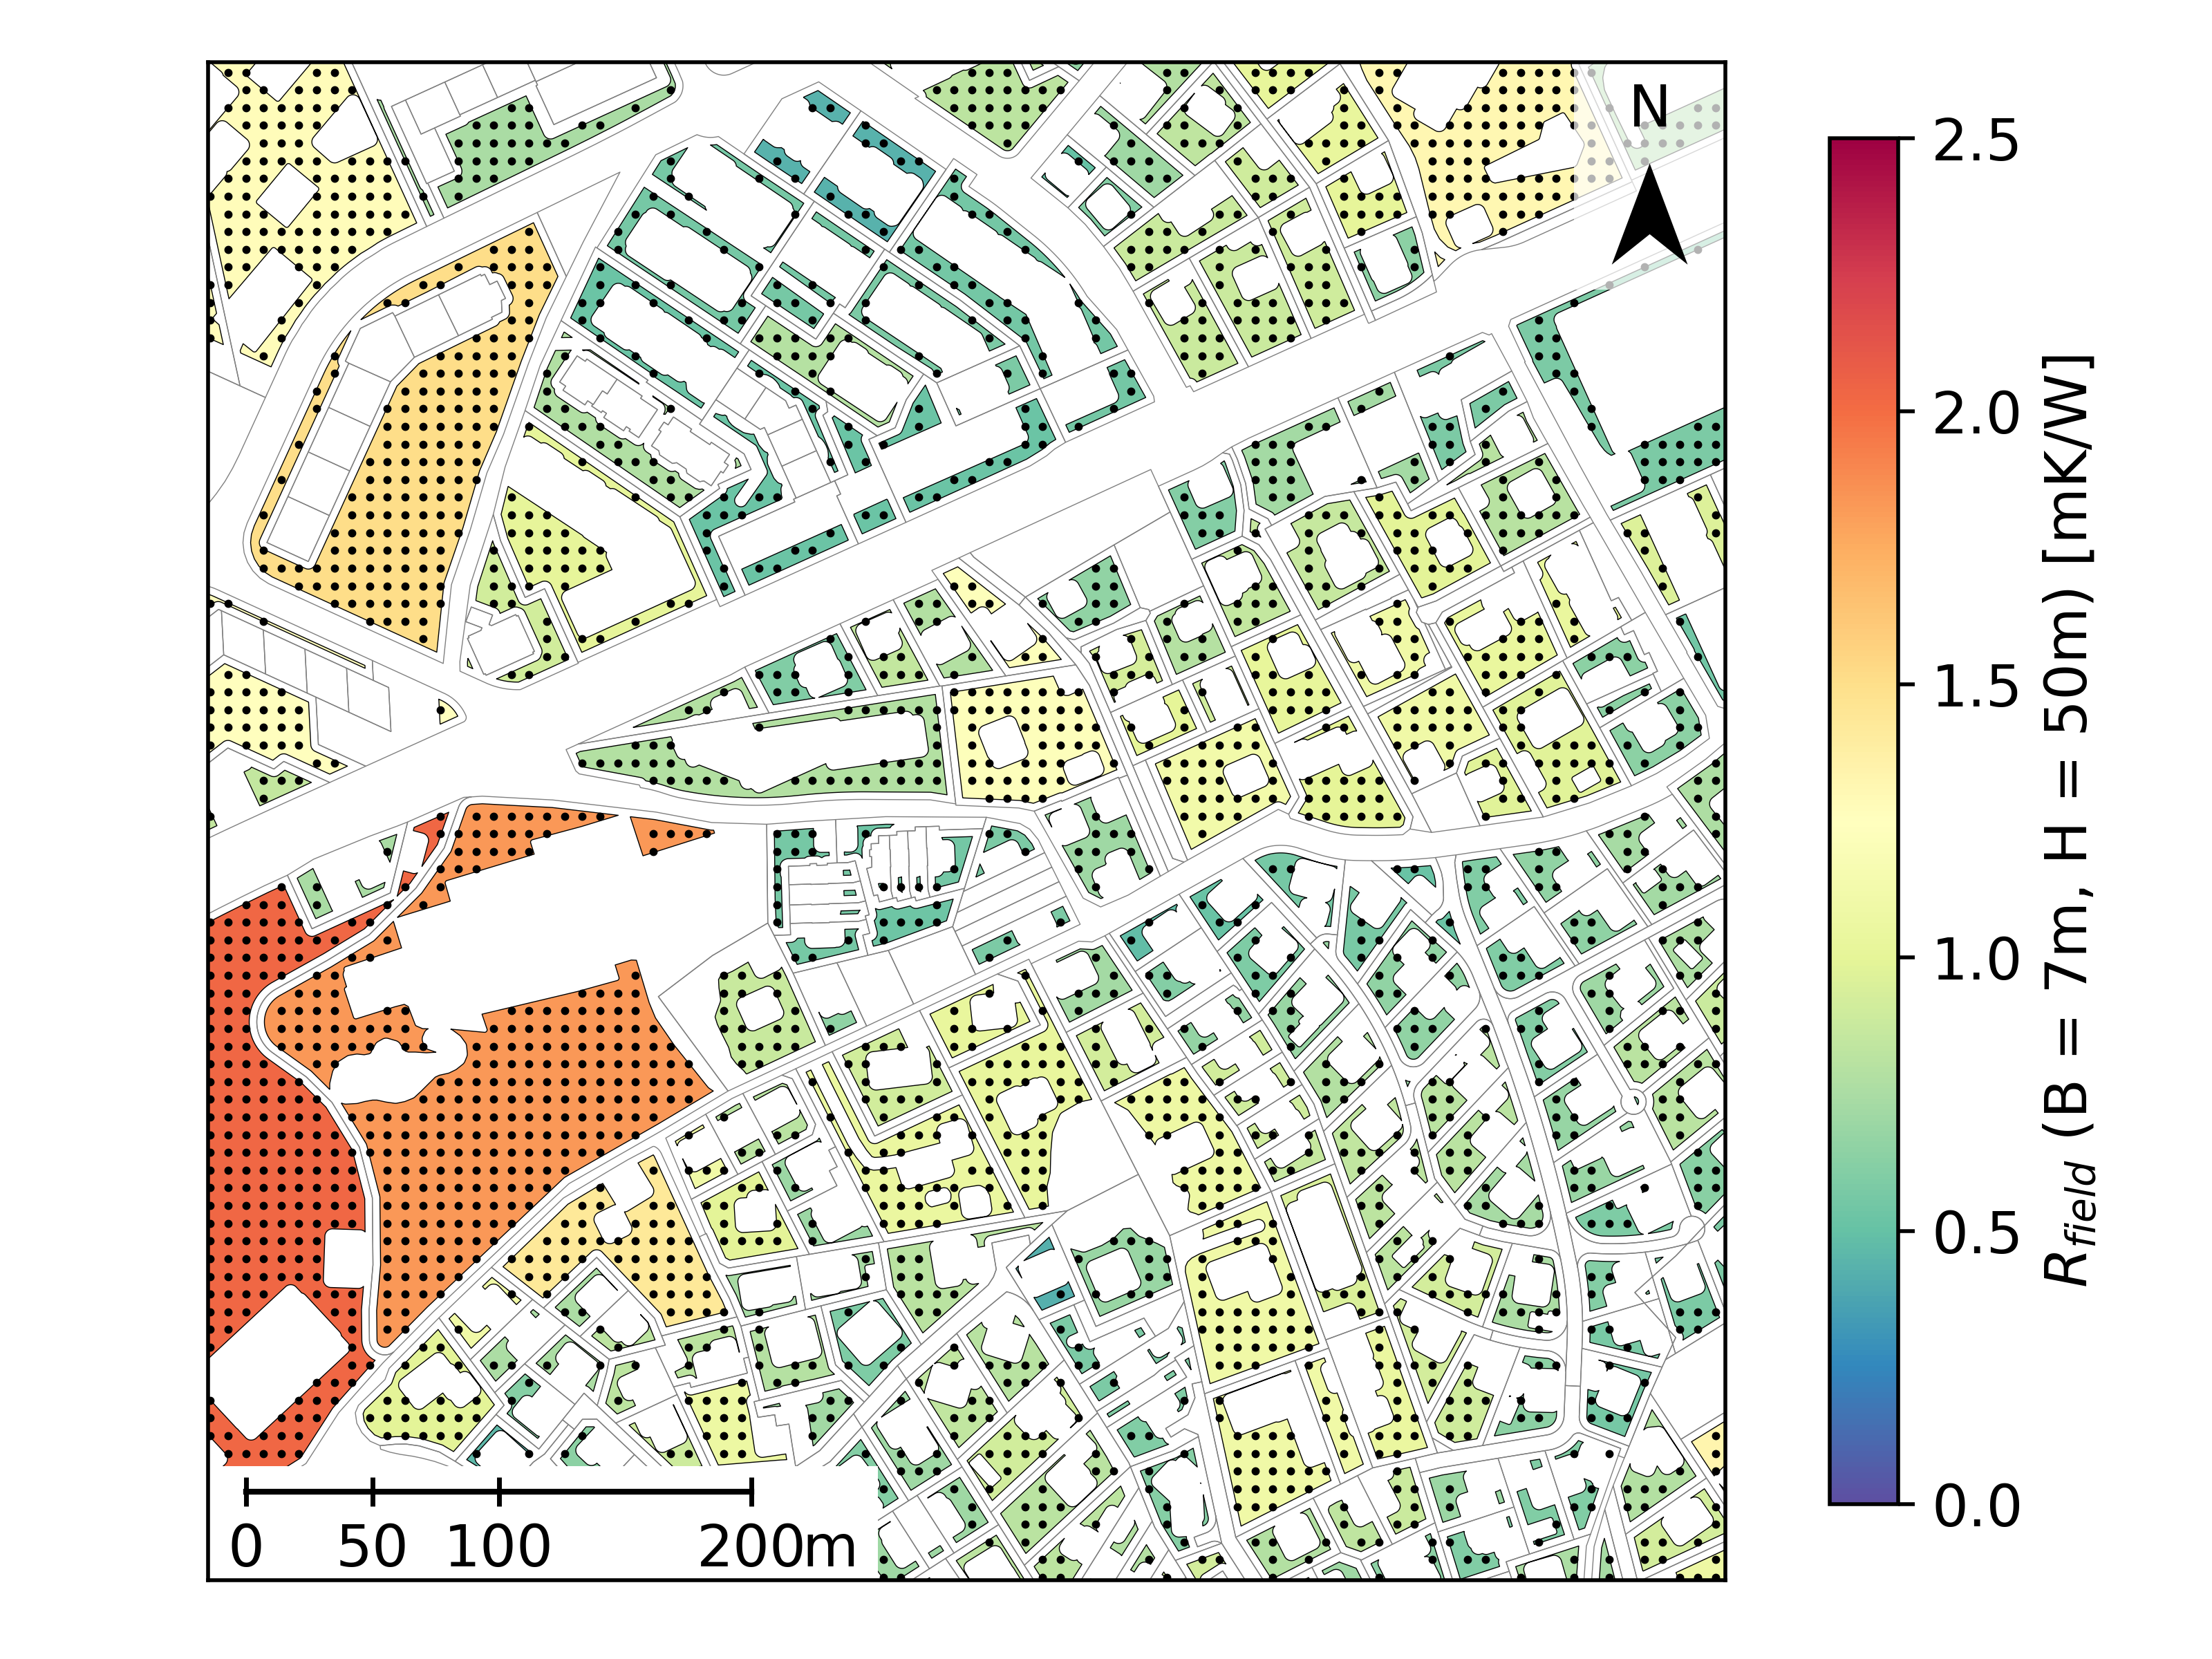
\includegraphics[width=.9\linewidth]{Figs/R_field_7_50_w_BHEs_V5_Tg1_HDD_newMargin.png}  
  \subcaption{}
  \label{fig:R_field_sample}
\end{subfigure}
\begin{subfigure}{.49\textwidth}
  \centering
  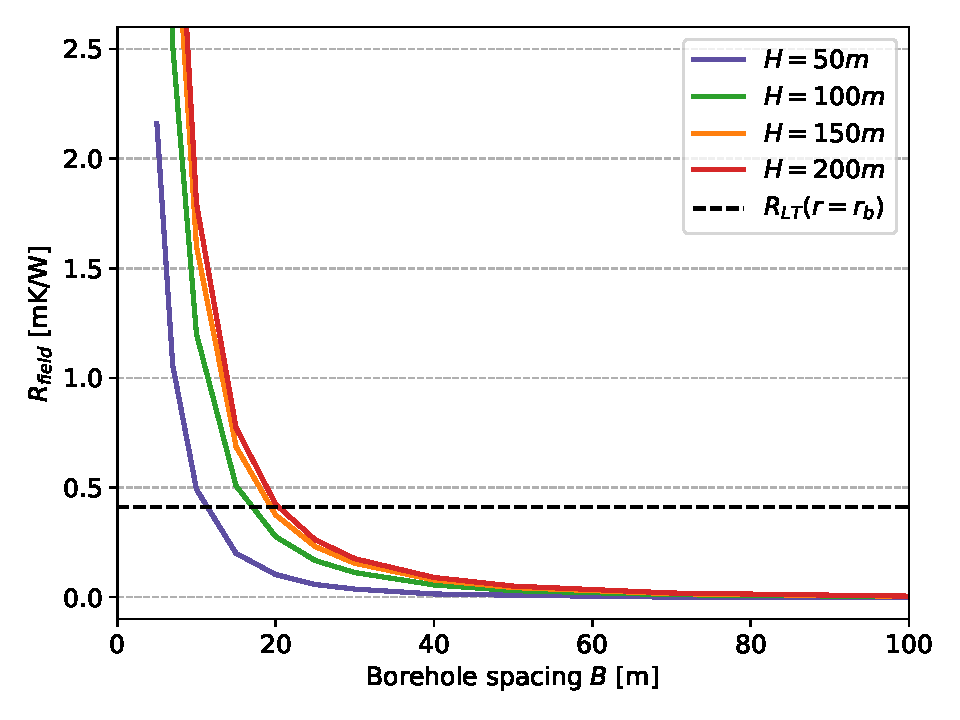
\includegraphics[width=.9\linewidth]{Figs/R_field_V5_Tg1_HDD_newMargin.pdf} 
  \subcaption{}
  \label{fig:R_field_mean}
\end{subfigure}
}
\caption{a) Sample of borehole fields for a suburban area near Geneva, showing the potential BHEs for $B = 7m$ (black dots) and the corresponding thermal resistance $R_{field}$ (colour gradient) at $H = 50m$, b) $R_{field}$ for each scenario of $B$ and $H$, averaged across all fields. The dashed line indicates the long-term resistance at the borehole wall ($R_{LT}(r=r_b)$), averaged for all $H$.}
\label{fig:R_field}
\end{figure}

\subsection{Optimisation and trade-offs}

The optimisation yielding the technical potential $Q_{pot}$ requires a trade-off between the heat extraction rate $q_{max}$ and the extractable energy $Q_{field}$, which is shown in Fig.~\ref{fig:optimisation}.
%
It indicates that $q_{max}$ (Fig.~\ref{fig:q_max}) increases with borehole spacing $B$ for all borehole depths $H$, while $Q_{field}$ (Fig.~\ref{fig:Q_field}) decreases with $B$ due to a lower number of installed BHEs ($N_B$).
Notably, $q_{max}$ decreases with $H$ for low $B$, but shows the opposite behaviour if $B$ is high.
The former is due to the lower $R_{field}$ of shallower BHEs (see Fig.~\ref{fig:R_field_mean}), while the latter is driven by a higher ground temperature at higher depths. 
%
The intersection of $q_{max}$ with the thresholds of 80\% of $q_{nom}$ (dashed lines in Fig.~\ref{fig:q_max}) suggests that the average $B_{opt}$ (dots) lies between $10-20m$, very close to the intersections of $R_{field}$ with $R_{LT}$ (see Fig.~\ref{fig:R_field_mean}). 
% The optimisation results yield an average $Q_{pot}$ of $55kWh$ and $40kWh$ in "permitted" and "limited" zones, respectively (with $H_{opt} = H_{max}$, excluding the highest and lowest $5^{th}$ percentiles).
The higher $q_{max}$ for low $H$ may in some cases outweigh the greater BHE depth, as the lower $R_{field}$ of shallow BHEs allows for a lower $B$. 
On average, this yields an equal potential for $H = 50m$ and $H = 100m$, and it may result in a choice of $H_{opt} < H_{max}$ in the optimisation.

% CHECK NUMBERS

\begin{figure}[ht!]
\centering
\begin{subfigure}{.49\textwidth}
  \centering
  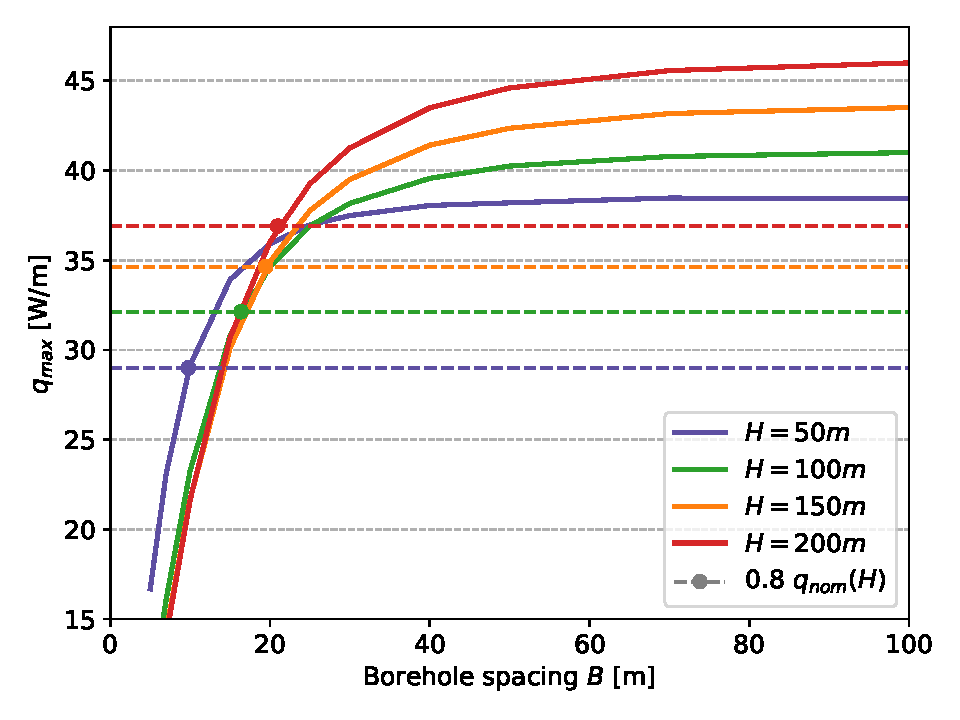
\includegraphics[width=\linewidth]{Figs/q_max_V5_Tg1_HDD_newMargin.pdf} 
  \subcaption{}
  \label{fig:q_max}
\end{subfigure}
\begin{subfigure}{.49\textwidth}
  \centering
  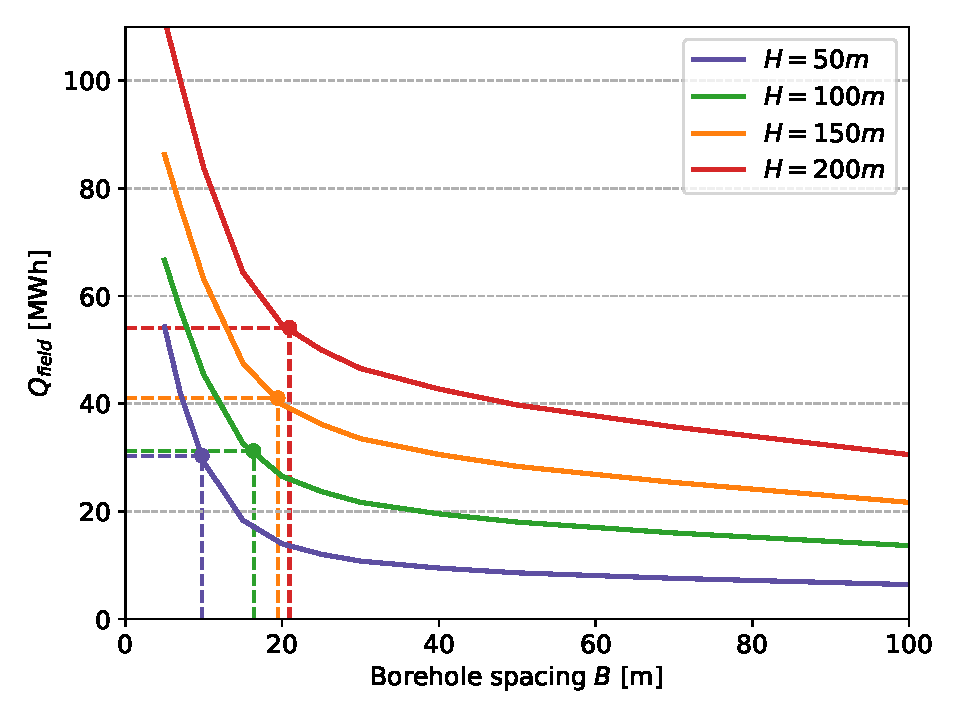
\includegraphics[width=\linewidth]{Figs/Q_field_no_outliers_V5_Tg1_HDD_newMargin.pdf} 
  \subcaption{}
  \label{fig:Q_field}
\end{subfigure}

\caption{Heat extraction rate $q_{max}$ (a) and  the corresponding extractable energy $Q_{field}$ (b) as a function of $B$ and $H$. 
The lines show averages across 90\% of the fields, excluding the lowest and highest $5^{th}$ percentile.
The dots in both figures indicate the intersection of $q_{max}$ with $0.8 \ q_{nom}$, which is the minimum accepted operating power for each $H$ shown as dashed line in (a).}
\label{fig:optimisation}
\end{figure}

The $B_{opt}$ and $H_{opt}$ resulting from the optimisation are shown in Fig.~\ref{fig:pixel_B_H}, averaged for each pixel of $200 \times 200m^2$. 
The average $B_{opt}$ ranges from $5-10m$ in urban areas to $30-40m$ in rural areas, where many large fields are located.
As large fields have, on average, a higher $R_{field}$ than small fields (see Fig.~\ref{fig:R_field_sample}), a higher spacing $B_{opt}$ is required to fulfill the optimisation constraints.
The $H_{opt}$ is close to the maximum value of $200m$ in the "permitted" zone but varies between $50-150m$ in the "limited" areas. 
As $H_{max} = 150m$ in the "limited" zone, the benefits of a relatively high $q_{max}$ frequently outweigh the additional energy gain from a higher $H$ (see Fig.~\ref{fig:optimisation}).
% The large spatial variations of the BHE arrangements within these ranges are due to the complex interactions between the theoretical potential, the available area and the design rules.

\begin{figure}[tb]
\centering
\makebox[\linewidth][c]{
\begin{subfigure}{.49\textwidth}
  \centering
  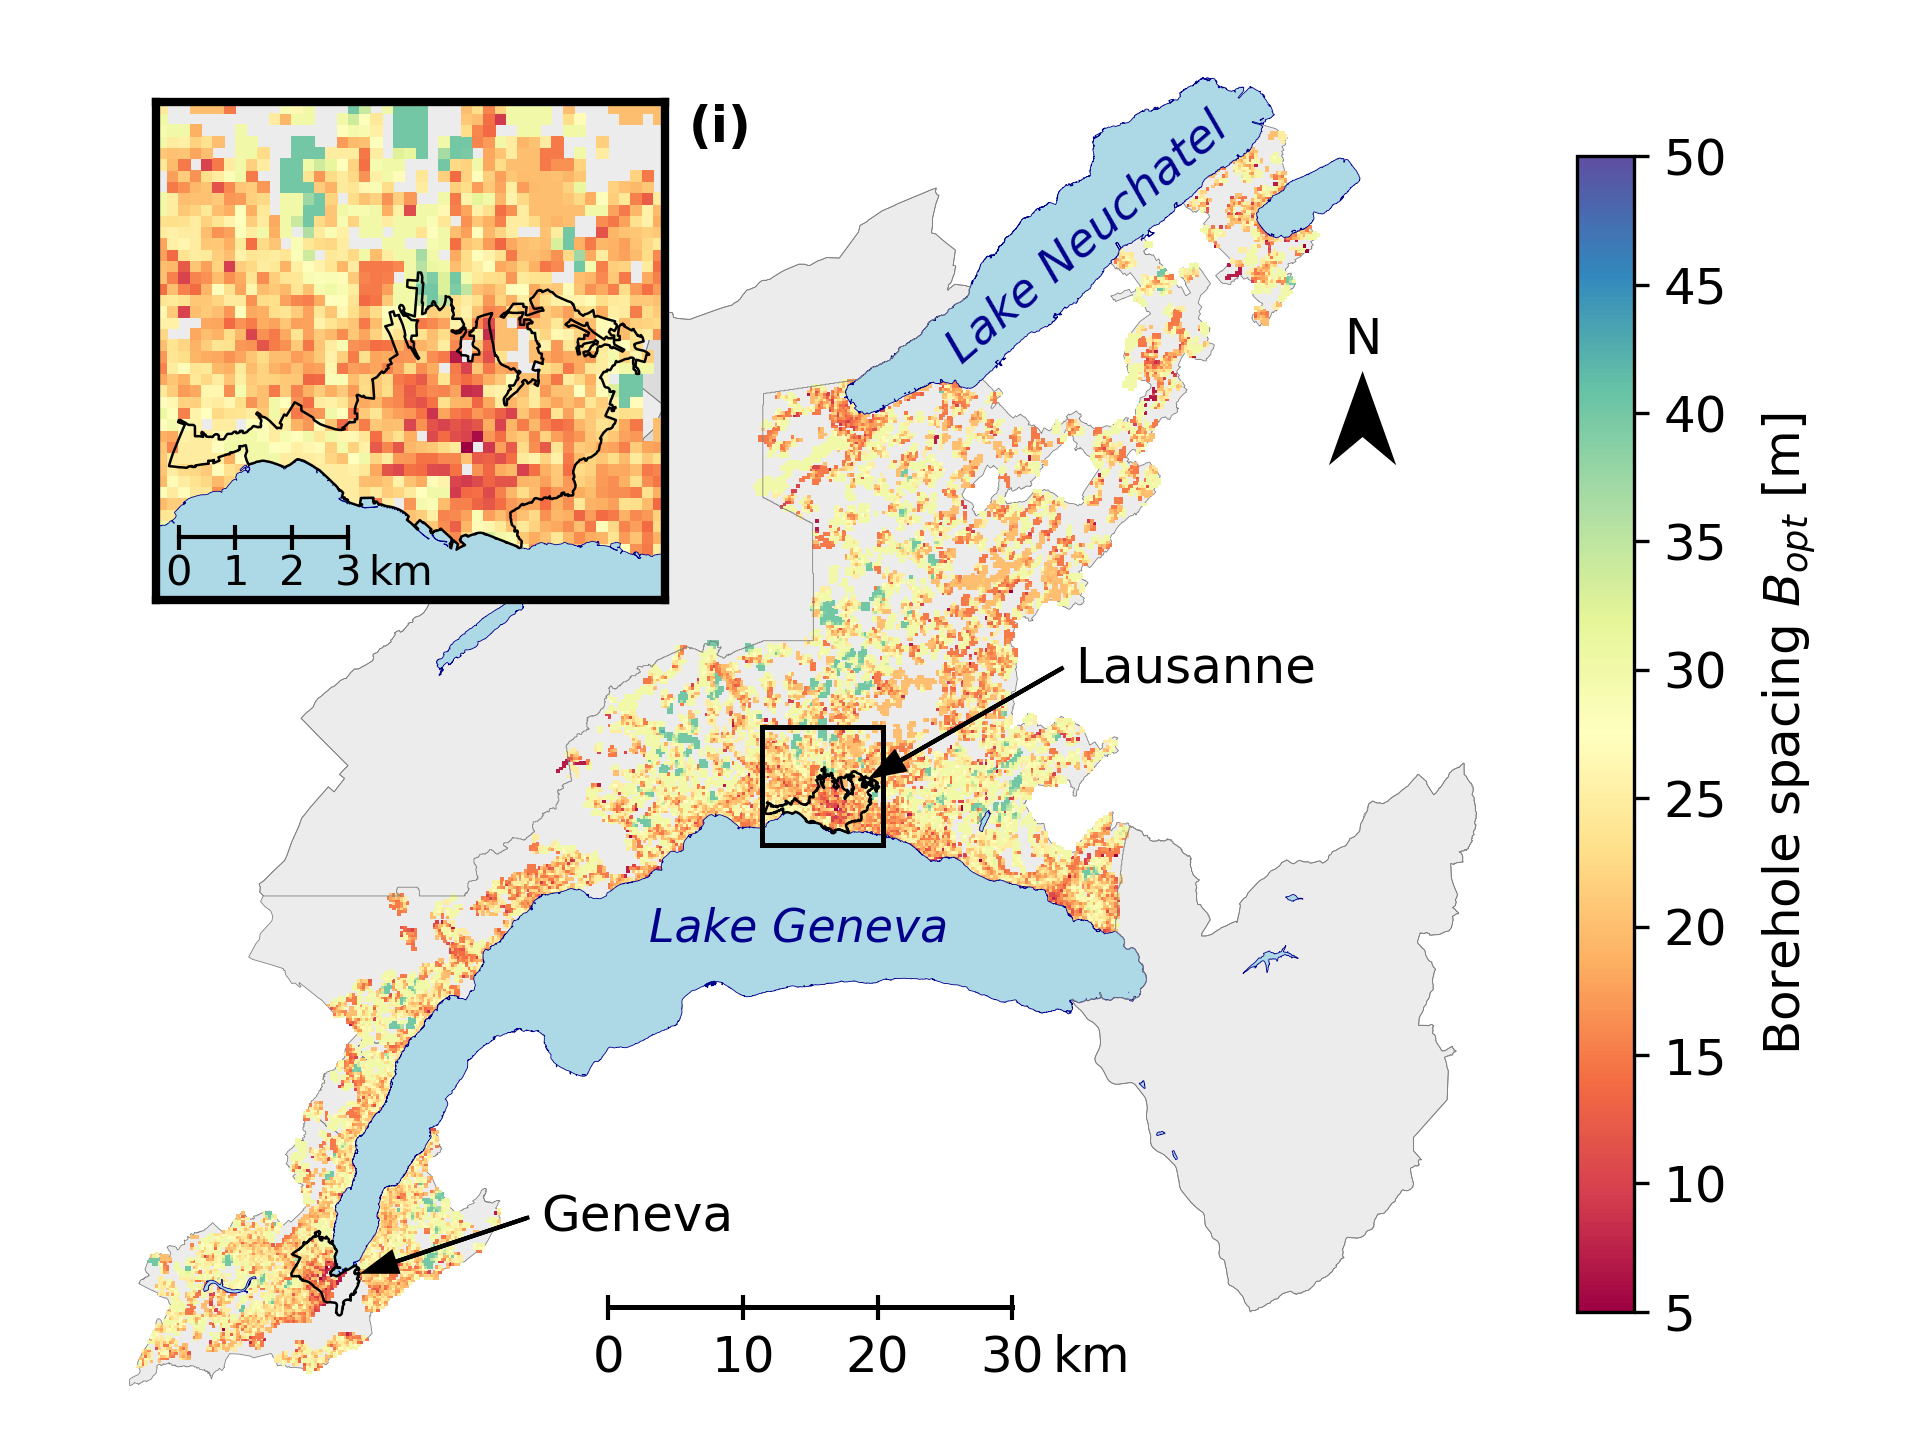
\includegraphics[width=\linewidth]{Figs/B_mean_V5_Tg1_HDD_newMargin.png}  
  \subcaption{}
  \label{fig:B_mean}
\end{subfigure}
\begin{subfigure}{.49\textwidth}
  \centering
  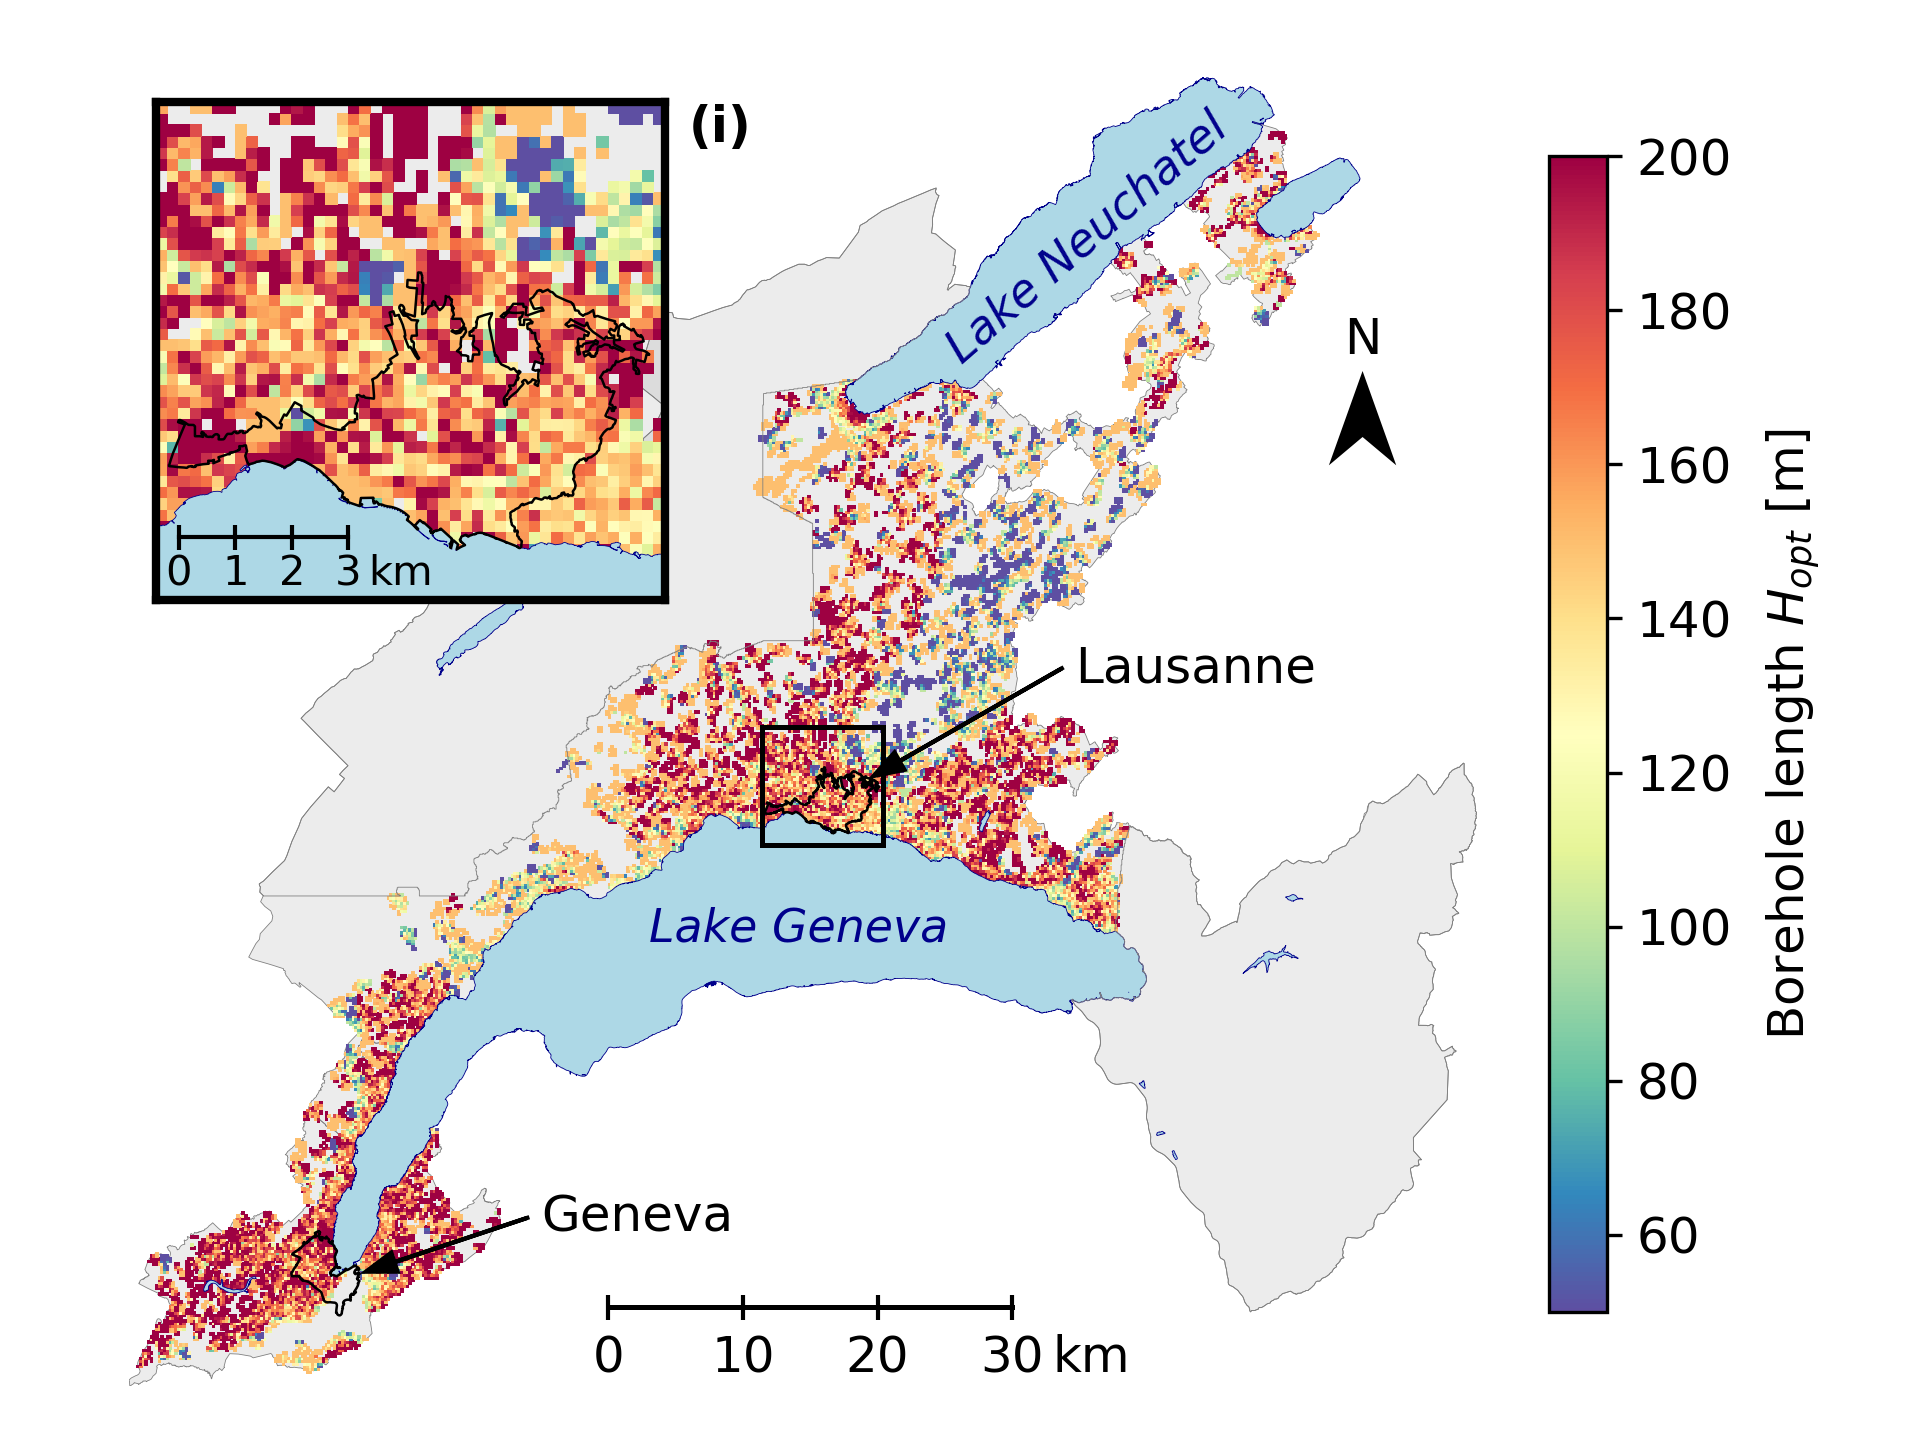
\includegraphics[width=\linewidth]{Figs/H_mean_V5_Tg1_HDD_newMargin.png} 
  \subcaption{}
  \label{fig:H_mean}
\end{subfigure}
}
\caption{a) Optimised borehole spacing $B_{opt}$ and b) borehole depth $H_{opt}$, both averaged across all BHEs within each $200 \times 200m^2$ pixel. The value for $B_{opt}$ accounts only for those fields with more than one BHE and represents the average per available area.}
\label{fig:pixel_B_H}
\end{figure}

The results further indicate that the optimal number of installed BHEs ($N_{B,opt}$, i.e. $N_B$ at $B = B_{opt}$) decreases with $H_{opt}$, as deeper BHEs frequently require a higher spacing to fulfil the optimisation constraints. 
As Fig.~\ref{fig:BHE_count_len} shows, the maximum $N_{B,opt}$ (blue line) decreases from 40 BHEs per hectare (corresponding to an average $B_{opt}$ of $15m$) for the shortest probes to 10 BHEs ($B_{opt} = 30m$) for $H_{opt} = 200m$. 
By contrast, the maximum cumulative BHE depth per hectare (red line) is approximately constant with $H_{opt}$, at just below $2 km / ha$ given a minimum borehole spacing of $5m$ and a maximum depth of $200m$. 
These findings suggest that the cumulative installed borehole depth per hectare may more suitable for constraining the dense deployment of BHEs than a minimum spacing between adjacent boreholes.
% To quantify this relationship at the scale of pixels of $200 \times 200 m^2$, we assess the optimal number of installed BHEs ($N_{B,opt}$, i.e. $N_B$ at $B = B_{opt}$) as a function of $H_{opt}$, shown in Fig.~\ref{fig:BHE_count_len} for all pixels (dots).
%
% The $N_{B,opt}$ decreases from 40 BHEs per hectare (corresponding to an average $B_{opt}$ of $15m$) for the shortest probes to 10 BHEs ($B_{opt} = 30m$) for $H_{opt} = 200m$. 

\begin{figure}[tb]
\centering
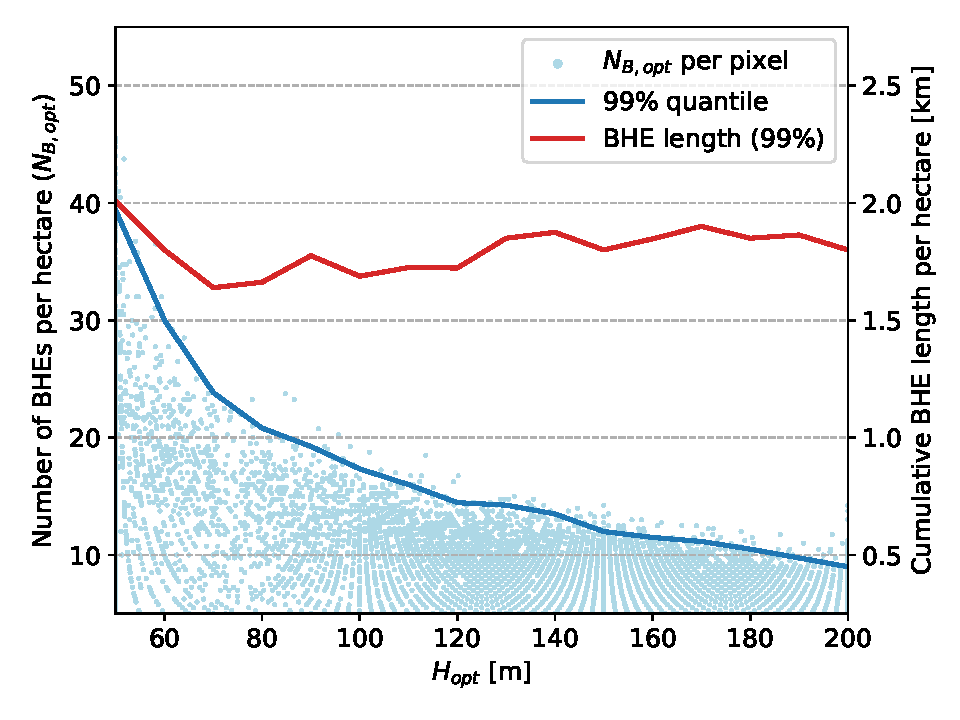
\includegraphics[width=0.6\linewidth]{Figs/BHE_count_length_V5_Tg1_HDD_newMargin.pdf} 
\caption{Optimal number of boreholes ($N_{B,opt}$) per hectare for all $200 \times 200m^2$ pixels (dots). The blue line marks the $99^{th}$ percentile per average depth $H_{opt}$ ($10m$ bins). The red line shows the corresponding cumulative installed BHE depth, given by $N_{B,opt} \times H_{opt}$ (right axis). The normalization per hectare is chosen for reasons of interpretability.}
\label{fig:BHE_count_len}
\end{figure}


\subsection{Technical geothermal potential}

The technical potential (Fig.~\ref{fig:Q_pot}) yields an annual total of $4.65 TWh$ for all parcels, or $16.4 kWh/m^2$ of available area ($284 km^2$). 
Most of the parcels ($\sim 60 \%$) are fitted with one or two BHEs, frequently in gardens of private properties (see Fig.~\ref{fig:Q_pot_sample}). 
%
Those of a shallow depth ($\leq 100m$) yield less than $15 MWh$, while deeper BHEs, $\geq 150m$, may provide up to $35 MWh$ per field. 
How boreholes are arranged in larger fields ($> 2$ BHEs) depends on the shapes and sizes of the fields. 
For example, narrow fields have a small thermal influence from adjacent BHEs, which results in a maximum potential for shallow and closely spaced (here $10m$) boreholes.
The influence of surrounding BHEs is highest for fields of rectangular shape, leading to a larger spacing (here $30m$) and the maximum depth. 
Few parcels ($\sim 2 \%$) are very large and may fit more than 60 BHEs, which exceeds the maximum existing field size in the region. If all fields are capped to this value, the annual potential reduces to $4 TWh$.
% THIS COULD GO IN THE DISCUSSION

The variation of the energy density, defined as the technical potential per unit area (Fig.~\ref{fig:Q_pot_pixel}), ranges from $2 kWh/m^2$ to $15.5 kWh/m^2$. 
The highest energy density is found in the urban and suburban areas at the borders of the lakes of Geneva and Neuchâtel ($\sim 30 \%$ of available area) and in rural areas with an available area percentage near 100\%. 
In the city centers of Lausanne and Geneva, the energy density is low despite the high $H$ and low $B$, as the available area is small ($< 10\%$).
Furthermore, the area in the north-east of Lausanne is characterised by a lower potential. This zone has a lower surface temperature (see Fig.~\ref{fig:T0}), which reduces the total allowed temperature drop. 

\begin{figure}[tb]
\centering
\makebox[\linewidth][c]{
\begin{subfigure}{.49\textwidth}
  \centering
  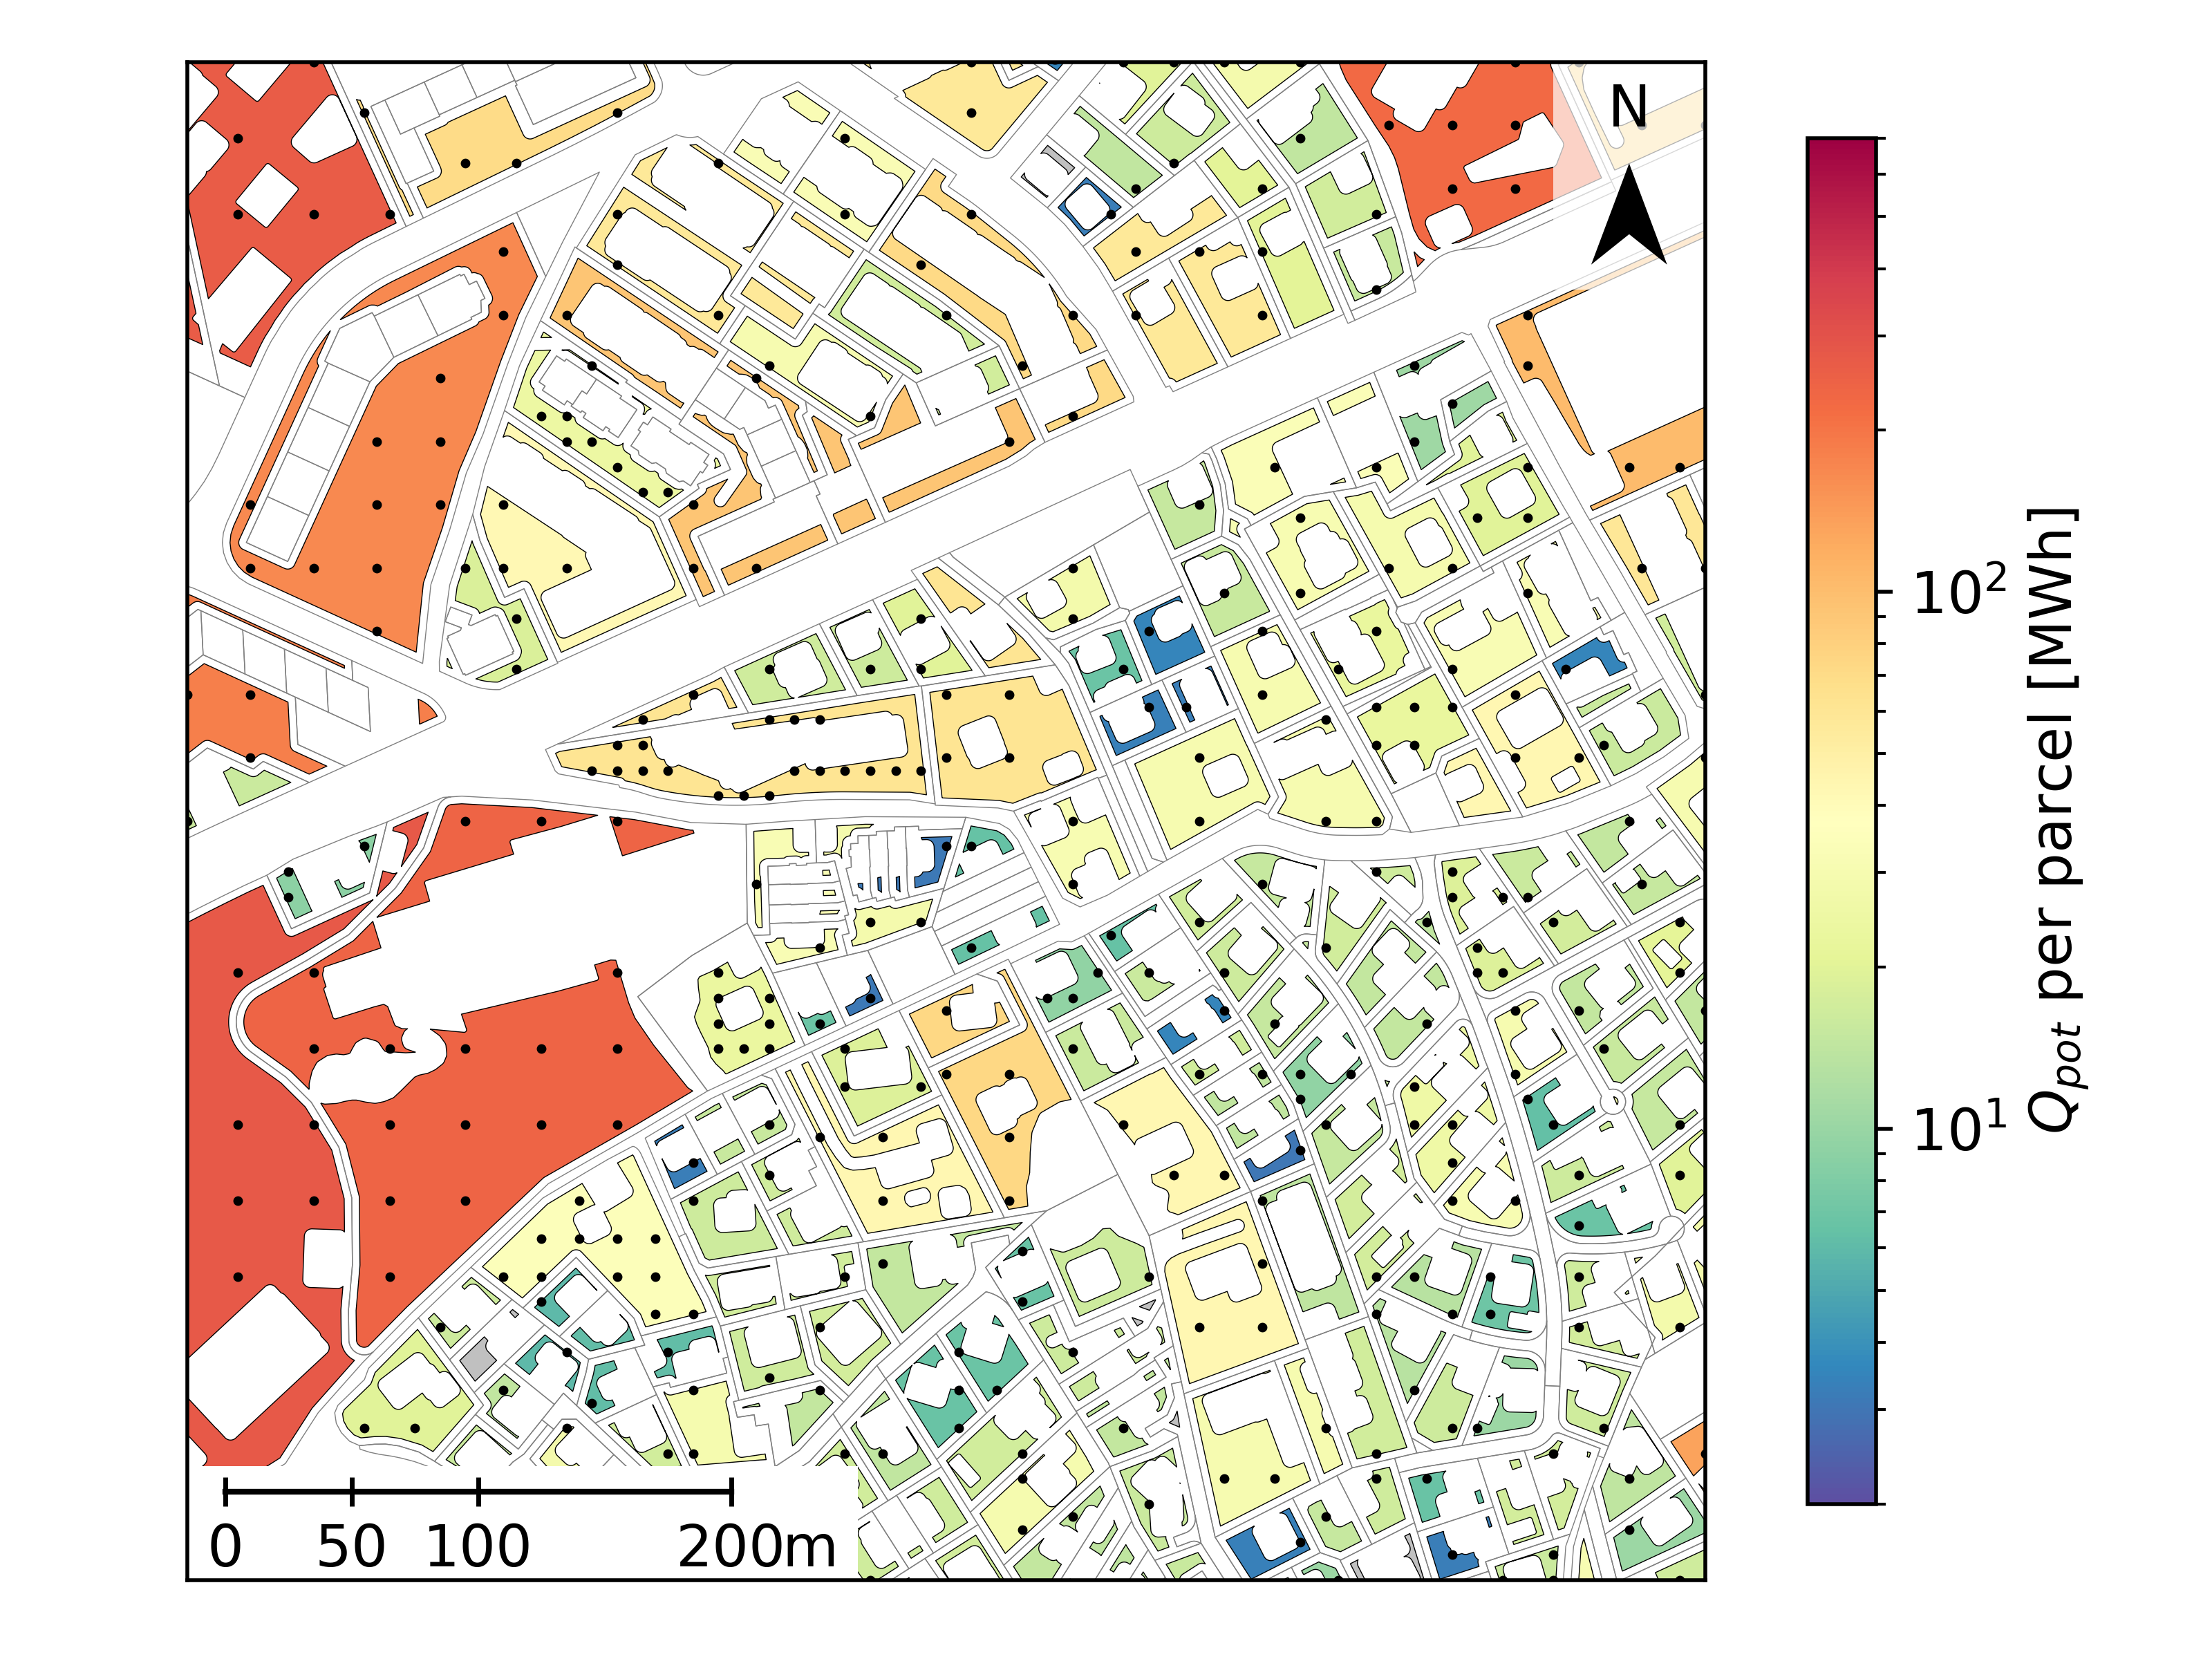
\includegraphics[width=.9\linewidth]{Figs/Q_pot_sample_V5_Tg1_HDD_newMargin.png}  
  \subcaption{}
  \label{fig:Q_pot_sample}
\end{subfigure}
\begin{subfigure}{.49\textwidth}
  \centering
  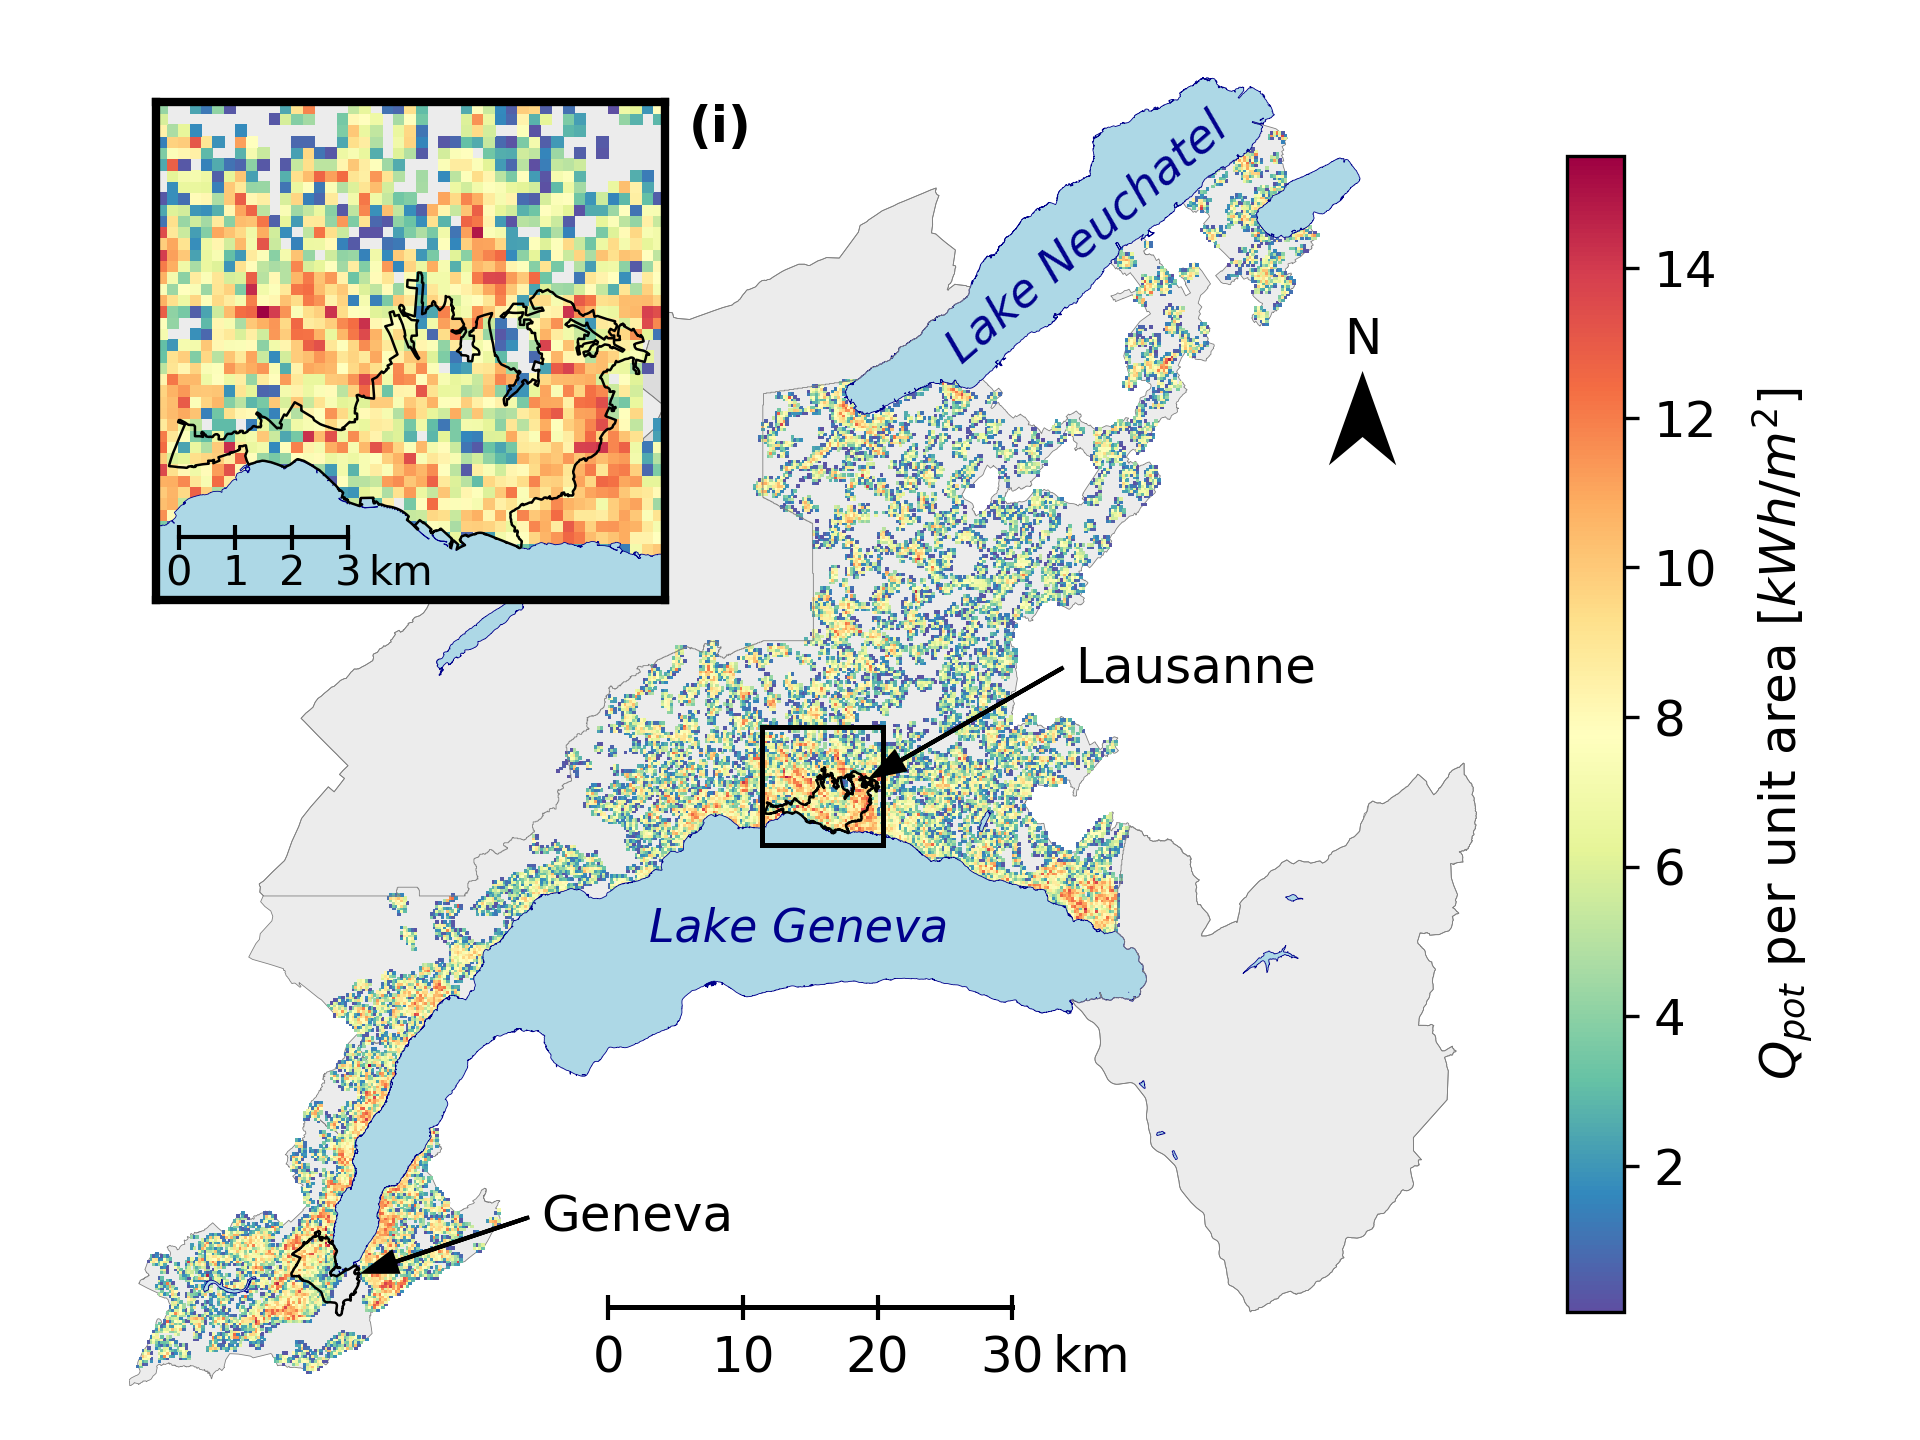
\includegraphics[width=\linewidth]{Figs/Q_pot_per_area_V5_Tg1_HDD_newMargin.png} 
  \subcaption{}
  \label{fig:Q_pot_pixel}
\end{subfigure}
}
\caption{a) Annual technical potential $Q_{pot}$ (in $MWh$) for the sample area (coloured fields), with the optimised BHE locations (dots), b) $Q_{pot}$ per unit area (in $kWh/m^2$) for pixels of $200 \times 200m^2$.} 
\label{fig:Q_pot}
\end{figure}

In contrast to the technical potential, the energy demand is strongly concentrated in urban areas and exceeds $1 MWh/m^2$ in the centers of Lausanne and Geneva, as shown in Fig.~\ref{fig:demand}. 
This leads to a large local energy deficit in these areas (Fig.~\ref{fig:deficit}), where complementary sources of renewable heat are indispensable.
In most rural areas, however, the energy demand can be covered fully by BHEs, and partially excess generation may be possible. 

\begin{figure}[tb]
\centering
\makebox[\linewidth][c]{
\begin{subfigure}{.49\textwidth}
  \centering
  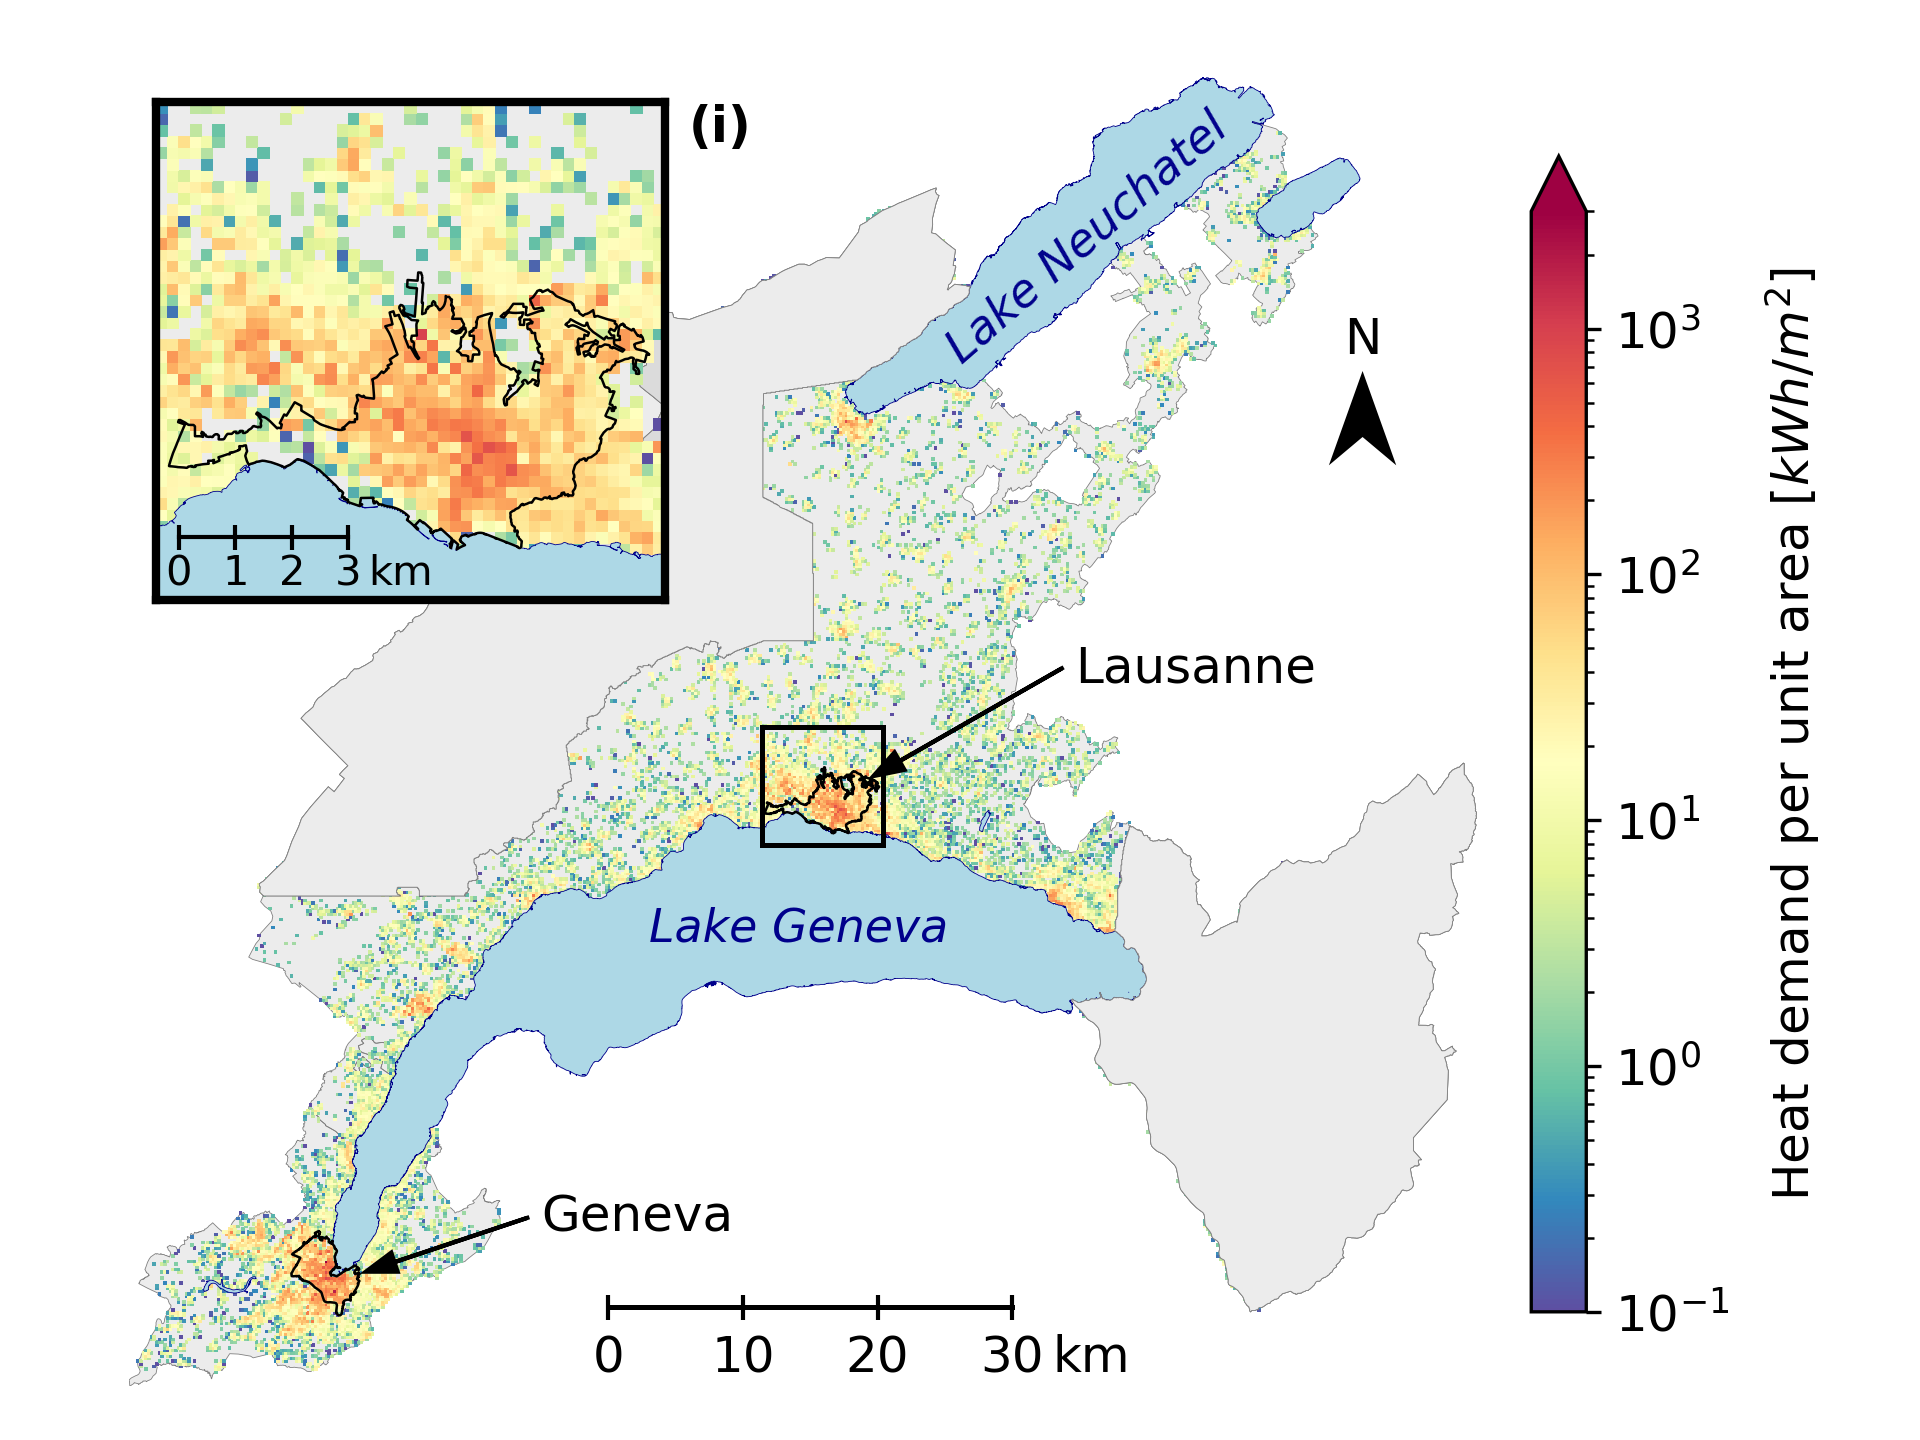
\includegraphics[width=\linewidth]{Figs/Q_demand_per_area.png}  
  \subcaption{}
  \label{fig:demand}
\end{subfigure}
\begin{subfigure}{.49\textwidth}
  \centering
  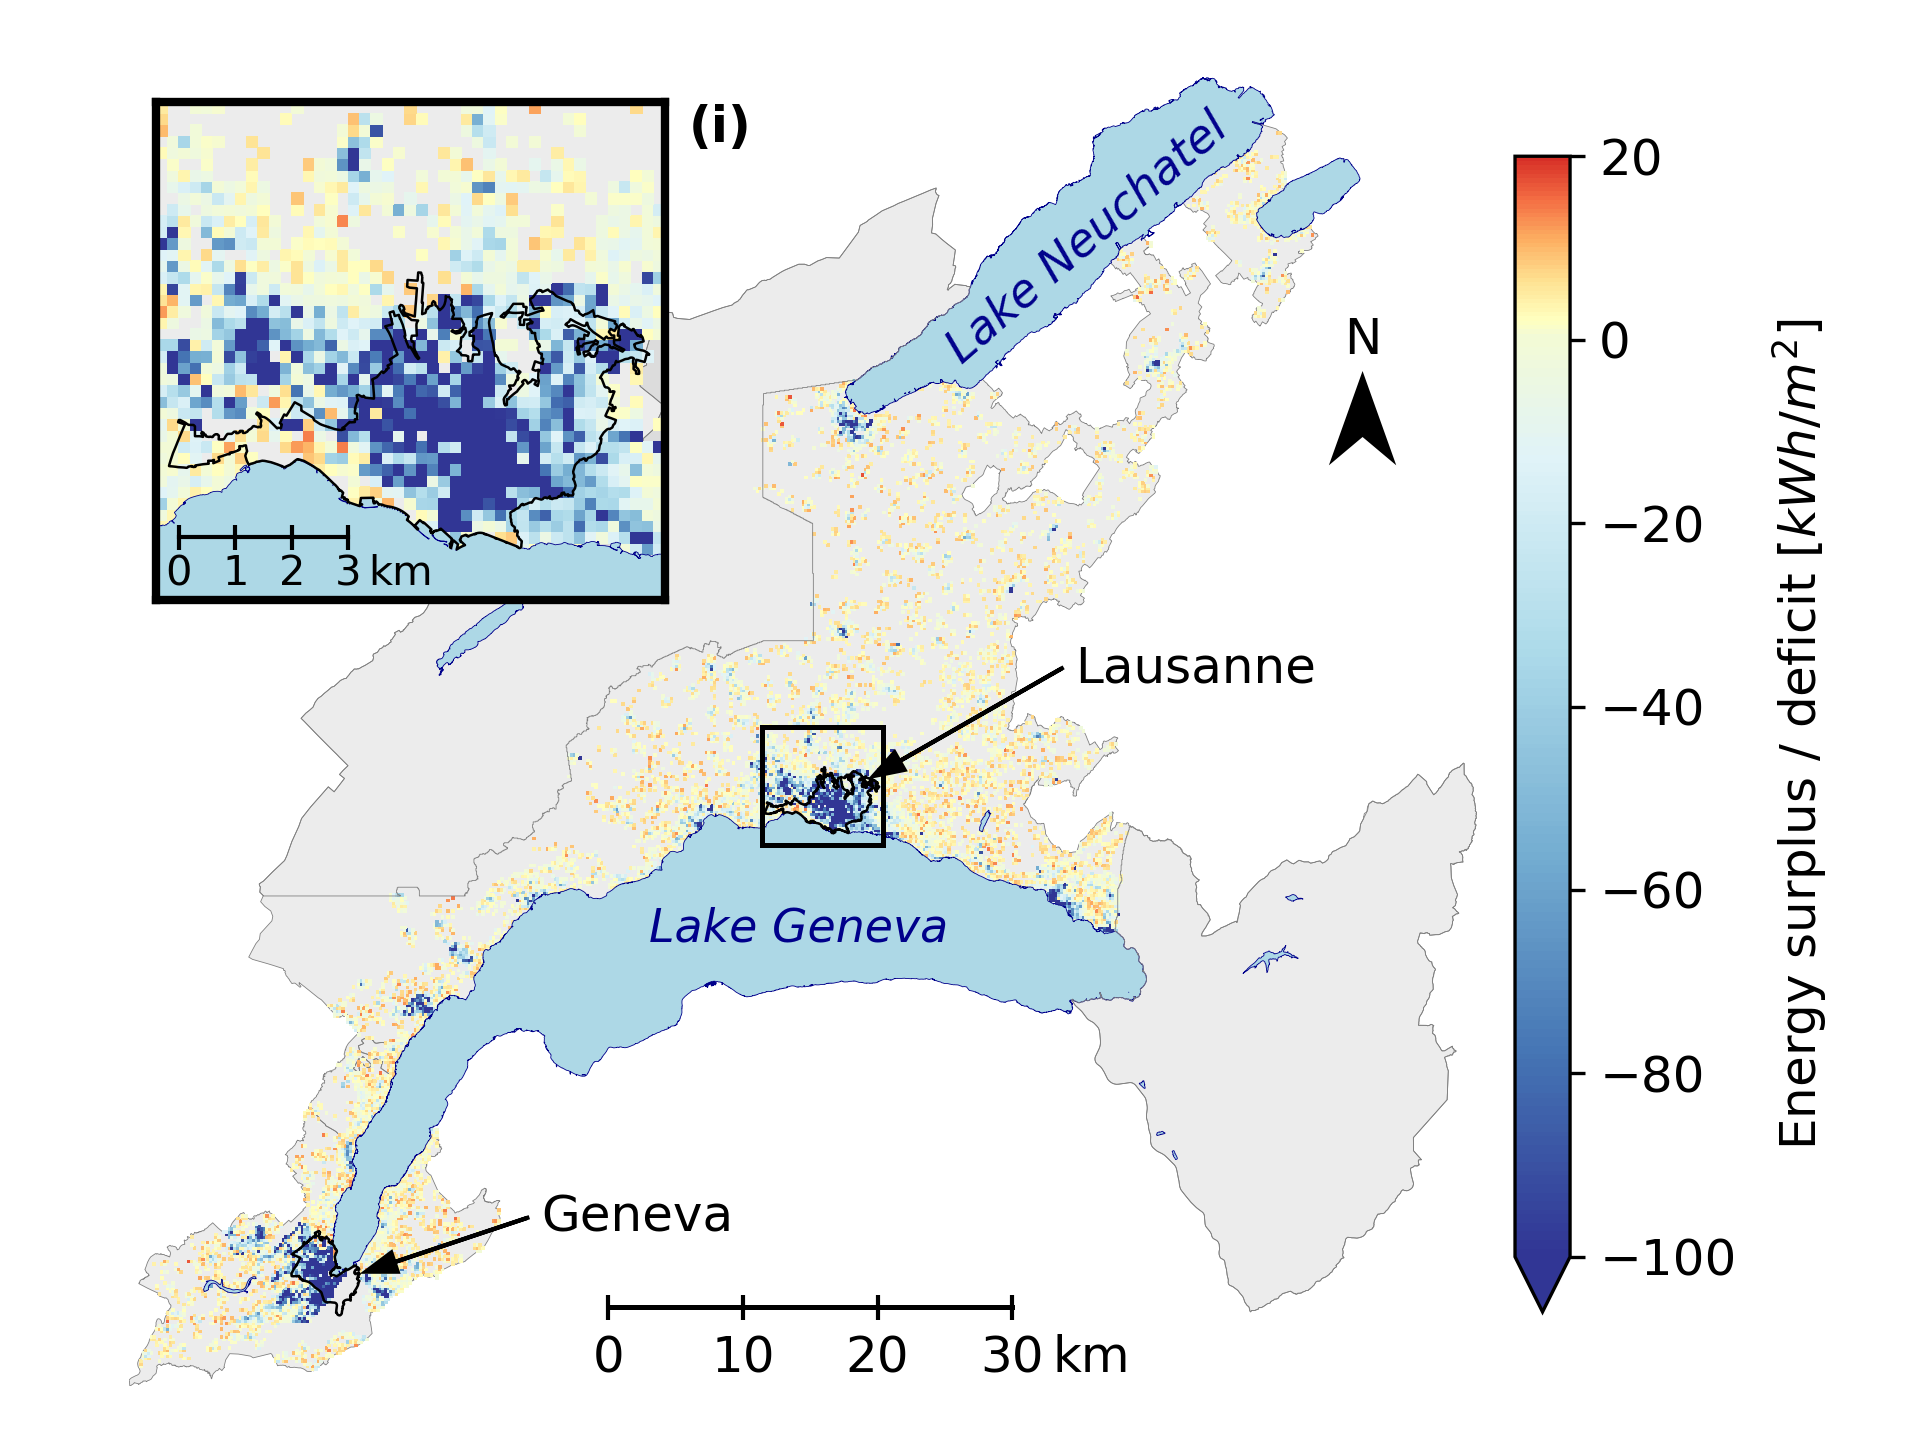
\includegraphics[width=\linewidth]{Figs/deficit_per_area_V5_Tg1_HDD_newMargin.png} 
  \subcaption{}
  \label{fig:deficit}
\end{subfigure}
}
\caption{a) Annual heat demand density (logarithmic scale) for pixels of $200 \times 200m^2$, according to \citet{schneider_spatialtemporal_2017}, b) Surplus (positive) or deficit (negative) of potential heat extraction from BHEs compared to the heat demand.}
\label{fig:demand_cover}
\end{figure}

\subsection{Sensitivity analysis}

The sensitivity analysis of the main input parameters ($\lambda$, $\alpha$, $T_0$, $\delta T/\delta z$, $t_{op}$, $r_b$, $R_b$) suggests that the energy potential of individual fields is, on average, most sensitive to $T_0$ and $\lambda$, followed by $t_{op}$ and $R_b$ (see Fig.~\ref{fig:sens_Q}). 
Accounting for the regional variation of these parameters (except $R_b$) with the highest possible accuracy is therefore essential to obtain a realistic potential estimate.
Furthermore, the estimation is sensitive to uncertainties in these values, which may arise from small-scale deviations and measurement errors, as well as from parameter variations due to different technologies and operation strategies. 
The sensitivity of $\alpha$, $r_b$ and $\delta T/\delta z$ is low, so the use of standard values based on the literature is justified. 

The results are exploratory and aim at providing an indication of the importance of each parameter on the technical potential. 
The change in $Q_{field}$ is obtained by varying each parameter separately around the average input data (see Table~\ref{tab:data}) and for the average BHE arrangement ($H = 150m, B = 20m$, 8 neighbouring boreholes). 
While Fig.~\ref{fig:sens_Q} shows the average sensitivity of $Q_{field}$ in the context of this case study, the results depend on the exact borehole arrangements and operation strategies.

The technical potential of GSHPs is further sensitive to the selected optimisation constraints, namely $q_{min}$ (percentage of $q_{nom}$) and $H_{max}$.
As Fig.~\ref{fig:sens_thresh} shows, the total technical potential decreases linearly with $q_{min}$ and increases over-proportionally with $H_{max}$, following the results from Fig.~\ref{fig:optimisation}.
The $Q_{pot}$ may hence be increased by accepting a lower minimum operating power or by increasing the maximum drilling depth. 
Doubling the potential for the given $H_{max}$ (dashed line in Fig.~\ref{fig:sens_thresh}) would for example  require dropping $q_{min}$ to only 50\% of $q_{nom}$.
Notably, the impact of $H_{max}$ on $Q_{pot}$ decreases with $q_{min}$ and becomes insignificant when $q_{min} = q_{nom}$, as the BHE arrangements converge to $H = 50m$, $B = 25m$ beyond 100\% of $q_{nom}$.
%This behaviour is caused by the decreasing average $H$ with increasing $q_{min}$, due to higher $H$ being infeasible, and a decreasing average number of BHEs per parcel. 
%These lead to a convergence of the BHE arrangements to $H = 50m$, $B = 25m$ beyond 100\% of $q_{nom}$.

\begin{figure}[tb]
\centering
\makebox[\linewidth][c]{
\begin{subfigure}{.49\textwidth}
  \centering
  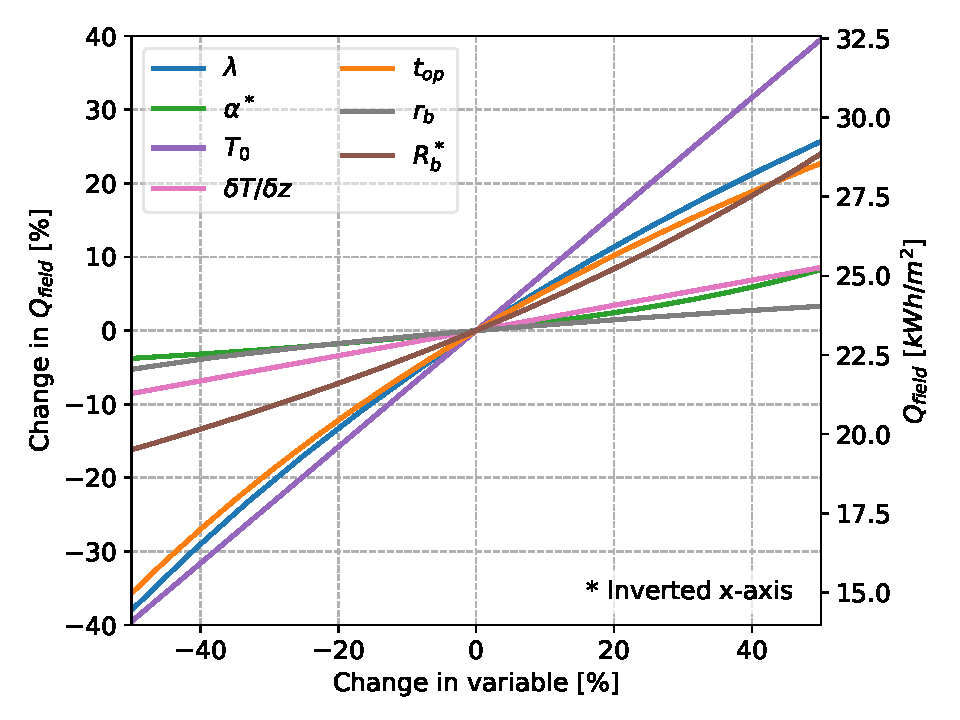
\includegraphics[width=.9\linewidth]{Figs/Sensitivity_Q_field_per_m2_print.pdf} 
  \subcaption{}
  \label{fig:sens_Q}
\end{subfigure}
\begin{subfigure}{.49\textwidth}
  \centering
  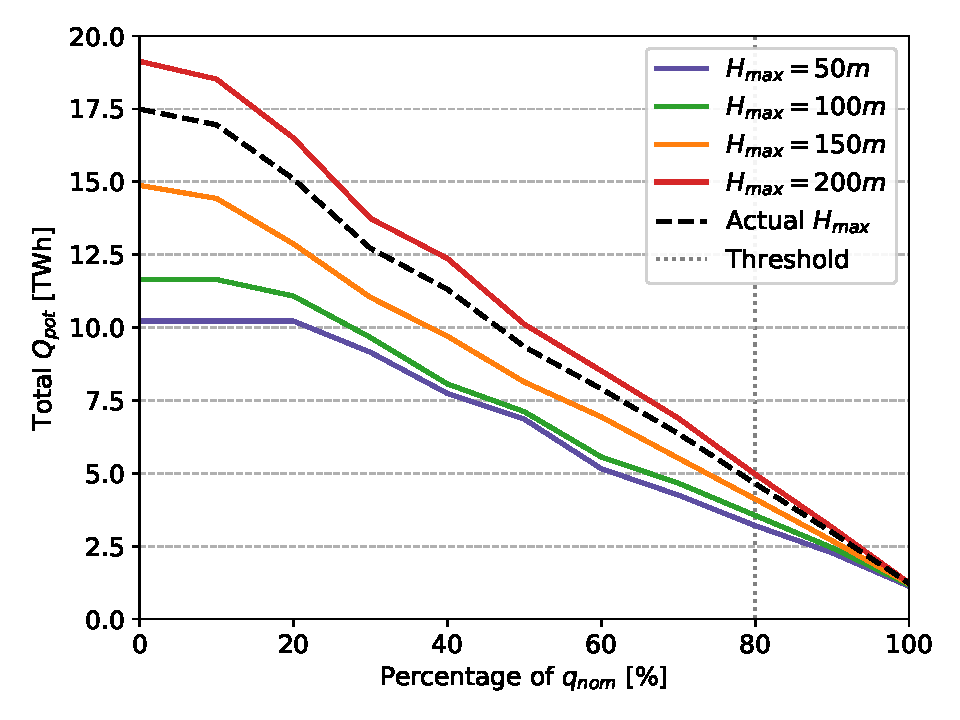
\includegraphics[width=.9\linewidth]{Figs/sensitivity_q_thresh_large.pdf} 
  \subcaption{}
  \label{fig:sens_thresh}
\end{subfigure}
}
\caption{a) Sensitivity of $Q_{field}$ to changes in the ground data ($\lambda$, $\alpha$, $T_0$, $\delta T / \delta z$) and the technical parameters ($t_{op}$, $r_b$, $R_b$). The change in $Q_{field}$ is computed by varying each parameter around the average values in Table \ref{tab:data} for the average BHE arrangement of $H=150m$, $B=20m$ and 8 neighboring boreholes.
b) Sensitivity of the technical potential $Q_{pot}$ to changes in the required heat extraction rate (x-axis) and in $H_{max}$ (colours), summed across all fields. The dashed line shows the varying $H_{max}$ used here.}
\label{fig:sensitivity}
\end{figure}

%%%%%%%%%%%%%%%%%%%%%%%%%%%%%%%%%%%%%%%%%%%%%%%%%%%%%%%
%%%%%%%%%%%%%%%%%%%%%%%%%%%%%%%%%%%%%%%%%%%%%%%%%%%%%%%

\section{Discussion}
\label{discussion_BHE}

\subsection{Methodological contribution}

Here we propose a novel approach for estimating the technical potential of GSHPs at regional scale, taking into account the available area for the installation of BHEs as well as the thermal interactions between boreholes.
%
The strength of our method lies in the combination of GIS and analytical modelling to simulate the potential effects of a dense deployment of BHEs for multiple scenarios of borehole spacing and depth.
As we derive the energy potential for each scenario from the maximum operating power under current installation standards, the estimation is independent of the energy demand.
%
The scenarios provide insights into the trade-off between energy and operating power, which is exploited in an optimisation step to suggest an optimised arrangement of BHEs for each individual parcel. 
% 
The spatial resolution of individual parcels allows to assess the impact of parcel shape, size and location on the technical potential, while the regional scale of the study highlights the variation of the technical potential in urban and rural areas.
% as well as the impact of the theoretical potential.

%%%%%%%%%%%%%%%%%%%%%%%%%%%%%%%%%%%%%%%%%%%%%%%%%

\subsection{Practical implications}

% FOR THE FIRST TIME
The case study in western Switzerland yields several practical contributions for a potential dense deployment of geothermal heat pumps. 
Firstly, we provide a regional-scale dataset of a technical potential of GSHPs
that accounts for interactions between boreholes and yields a potential of $4.65TWh$ on an available area of $284 km^2$.
Secondly, the aggregation to pixels of $200 \times 200 m^2$ highlights regional variations in the potential, which reaches up to $15.5 kWh/m^2$. 
According to our estimation, the potential is great enough to satisfy the heating demands in most rural and suburban areas but it is insufficient in urban centers, where complementary heat supplies would be needed.
Thirdly, our analysis suggests that the the cumulative installed borehole depth is a good indicator for the exploitation of the thermal capacity of the ground. 
In this case study, which assures at least 80\% of the nominal operating power for potential installations, the upper limit of cumulative depth is about $2km/ha$ given a minimum borehole spacing of $5m$ and a maximum borehole depth of $200m$. 
% ADD PART ON HEAT REJECTION / CONSERVATIVE ESTIMATE
%%%%%%%%%%%%%%%%%%%%%%%%%%%%%%%%%%%%%%%%%%%%%%%%%%%%%%%

\subsection{Limitations}
\label{limitations_BHE}

As any study estimating a technical potential of GSHPs, the present work is subject to uncertainties related to the modelling approach and the data. 
% and assumptions and lacks a ground truth for validation. 
The primary source of uncertainty is related to the ground thermal properties ($\lambda,\alpha$), as the underlying 3D subsurface models are regional models and may deviate from measured thermal properties in some locations. 
Such local deviations can only be assessed through test drillings.

This work is limited by some assumptions:
(i) the entire available area is considered suitable for installing BHEs. 
In practice, alternative uses of the subsurface such as utility lines, subways or tunnels may reduce the available area for geothermal installations \cite{li_integrated_2016}.
(ii) All BHE arrangements are based on rectangular grids covering the full area. 
The BHE arrangements suggest borehole numbers and depths that maximise the energy potential in the context of a dense deployment of BHEs, and do not represent installation recommendations for specific parcels.
(iii) We focus on the technical aspects limiting a dense deployment of BHEs.
Other aspects, such as environmental consequences due to cooling of the shallow subsurface, are not addressed here.
(iv) We do not consider additional heat transfer from groundwater flow, which may impact the technical geothermal potential. 
(v) More specifically, we only consider heat extraction for space heating, which is the dominant use of GSHPs in Switzerland.
The estimated potential may increase if excess heat, for example from space cooling, is re-injected into the ground, as that would partly recharge the ground with heat.
For countries with similar yearly temperatures as Switzerland or lower, the amount of heat re-injected into the ground during the comparatively short hot summer periods is likely to be small in relation to the heat extracted from the ground during the much longer cool winter periods. The details of this impact will be explored in a future work.

As this work is, to the best of our knowledge, the first of its kind in the case study area, a frame of comparison is lacking. 
While the quality of the ground data may be assessed from thermal response tests, a validation of the thermal interference between boreholes is only possible for individual case studies that already exhibit a high density of BHEs. 
The relevance of such a validation approach however is limited, as real installations are dimensioned to satisfy a given demand, while it is the subject of this work to estimate the maximum possible energy generation.

%%%%%%%%%%%%%%%%%%%%%%%%%%%%%%%%%%%%%%%%%%%%%%%%%%%%%%%

\subsection{Applications and future work}
\label{application_BHE}

Applications for a regional-scale estimate of the technical potential of BHEs include the support of policy making, urban planning and the development of a framework for the regulation of new installations. 
As part of their renewable energy strategies, policy makers may provide financial support mechanisms for businesses, homeowners and energy providers to invest in GSHPs, knowing that these may cover significant fractions of the heat demand in suburban and rural areas. 

Urban planners can use the results (i) to estimate the potential of GSHPs in any neighborhood in the study region, (ii) to assess the potential of district heating networks for transporting heat from areas with surplus generation to those with a deficit and/or (iii) to perform techno-economic analyses that compare GSHPs to alternative heat sources.
Local authorities may use the outcome from the proposed method to explore the limiting factors for a dense deployment of BHEs and to formulate guidelines to avoid an over-exploitation of the ground.
% , for example by developing a standard for the maximum cumulative borehole depth per hectare.

Future work will aim at the estimation of a technical geothermal potential at country scale.
This may be achieved by applying statistical methods such as Machine Learning, which have been used successfully to estimate the theoretical geothermal potential at national scale \cite{assouline_machine_2019}.
To further develop the proposed method, several limitations may be addressed, including the modelling of the additional heat transfer from groundwater flow, a systematic quantification of the uncertainties related to the data and the modelling approach and the impact of an active regeneration of the ground on the geothermal potential in dense urban areas.

%%%%%%%%%%%%%%%%%%%%%%%%%%%%%%%%%%%%%%%%%%%%%%%%%%%%%%%
%%%%%%%%%%%%%%%%%%%%%%%%%%%%%%%%%%%%%%%%%%%%%%%%%%%%%%%

\section{Conclusion}
\label{conclusion_BHE}

This work presents an estimation of the technical geothermal potential from shallow ground-source heat pumps for individual parcels at regional scale.
We define the technical potential as the maximum thermal energy that can be extracted from vertical borehole heat exchangers installed on all the available surface area, such that these can be operated with at least $80\%$ of the recommended operating power. 
The proposed method combines the ground thermal properties, the available area for borehole installation and the technical model of borehole heat exchangers and focuses on quantifying the thermal interference between boreholes, which has not previously been assessed at the regional scale.

The results provide a first estimate of the technical potential of borehole heat exchangers for a case study area in western Switzerland.
This estimate suggests that borehole heat exchangers may provide sufficient energy to cover the heat demand of most suburban and rural areas, while the potential is insufficient in dense urban centers.
Urban planners can use this data to assess the techno-economic aspects of a dense deployment of borehole heat exchangers.
Our findings further show that the cumulative installed borehole depth may be a suitable parameter to assess a potential over-exploitation of the heat capacity of the ground.
%
This work can contribute to the development of decarbonisation strategies for the heating sector in Switzerland by quantifying the potential for a renewable heat generation from shallow geothermal energy and by highlighting areas where complementary heat sources are needed.

% \section{Machine Learning for extrapolation to national scale}

\section{Potential for heating and cooling with ground regeneration}